% 2026-10-23：按学习复现、探索尝试、优化验证、迭代调试、整板尝试重组。
\documentclass[stage1,fontset=fandol]{ydzjreport}
\usepackage{subcaption,longtable}

\stageonesetup
{第 1 个逻辑月 · 学习与复现}
{冯旭东、陈思文}
{复合微通道分区冷却}
{【待确认】逻辑月 1 对应的自然月}
{软件学习；文献复现；初步小块理论；UDF 入门；自控基础}
{通过软件学习与文献复现建立研究基础，从非均匀热负荷提出初步小块思路；学习变物性和自控基础，开展 UDF 初步编写尝试。}
\pagestyle{empty}   % 去掉页眉与页脚（含页码）
\RemoveFromHook{enddocument}[ydzjreport] % 去掉末页的作者与格式规范收尾说明


\newlabel{sub@fig:repro-t}{{a}{4}{方形微通道温度\relax }{figure.caption.4}{}}
\newlabel{sub@fig:repro-p}{{b}{4}{方形微通道静压\relax }{figure.caption.4}{}}
\newlabel{sub@fig:repro-v}{{c}{4}{方形微通道速度大小\relax }{figure.caption.4}{}}
\newlabel{sub@fig:repro-cu}{{d}{4}{方形微通道铜板温度\relax }{figure.caption.4}{}}
\newlabel{sub@fig:h5-t}{{e}{4}{六边形微通道温度\relax }{figure.caption.4}{}}
\newlabel{sub@fig:h5-p}{{f}{4}{六边形微通道静压\relax }{figure.caption.4}{}}
\newlabel{sub@fig:h5-v}{{g}{4}{六边形微通道速度大小\relax }{figure.caption.4}{}}
\newlabel{sub@fig:h5-cu}{{h}{4}{六边形微通道铜板温度\relax }{figure.caption.4}{}}
\newlabel{sub@fig:circle-t}{{i}{4}{圆形微通道温度\relax }{figure.caption.4}{}}
\newlabel{sub@fig:circle-p}{{j}{4}{圆形微通道静压\relax }{figure.caption.4}{}}
\newlabel{sub@fig:circle-v}{{k}{4}{圆形微通道速度大小\relax }{figure.caption.4}{}}
\newlabel{sub@fig:circle-cu}{{l}{4}{圆形微通道铜板温度\relax }{figure.caption.4}{}}
\begin{document}
\section*{逻辑月1\_基础建立：图表附件}
本附件图表编号与对应提交正文及完整报告一致。\par\clearpage
\setcounter{table}{0}
\begin{table}[H]
	  \centering
	  \small
	  \renewcommand{\arraystretch}{1.12}
	  \caption{文献要点与研究思路}
	  \label{tab:notes}
	  \begin{tabularx}{\textwidth}{@{}>{\RaggedRight\arraybackslash}p{0.16\textwidth} Y Y@{}}
	    \toprule
\rowcolor{ydzjlight} 文献 & 论文要点 & 对小块思路及后续工作的启示 \\
	    \midrule
	    Ao 等\cite{ao} & 方形、圆形与六边形微通道的比较 & 复现三种流道，学习短流路与局部强化的组织方式 \\[3pt]
	    隋增光等\cite{ref1} & 综述数据中心吸收式器件散热、余热制冷、储能、发电与空气取水，强调低品位余热的多功能利用及系统集成。 & 补充研究背景与系统应用场景；在冷板研究之外，梳理出口水温、余热利用与节能节水之间的联系，拓展系统评价思路。 \\[3pt]
	    Xu 等\cite{ref2} & 针对双桥臂 SiC IGBT 多热源，研究双面液冷与六类导流微结构；海鸥形结构综合性能因子达 1.51，交错结构更利于芯片局部均温。 & 依据热源位置布置强化结构，将海鸥形、交错导流纳入候选矩阵；比较模块整体温度与局部热点温度，避免仅以平均温度筛选。 \\[3pt]

	    \bottomrule
	  \end{tabularx}
	\end{table}
\clearpage
\setcounter{table}{1}
\begin{table}[H]
	  \centering
	  \small
	  \renewcommand{\arraystretch}{1.12}
	  \caption{文献要点与研究思路（续1）}
	  \label{tab:notes-cont-2}
	  \begin{tabularx}{\textwidth}{@{}>{\RaggedRight\arraybackslash}p{0.16\textwidth} Y Y@{}}
	    \toprule
\rowcolor{ydzjlight} 文献 & 论文要点 & 对小块思路及后续工作的启示 \\
	    \midrule
	    Wang 等\cite{ref5} & 将非等高双层通道、分形分叉与冲击射流结合，并采用实验验证和 NSGA-II 优化；文中报告最优无肋方案的 PEC 较参照结构提高 24.61\%。 & 拓展“层间高度差—分叉配流—局部冲击”的组合方案；先比较不同进水组织，再开展热性能与压降的双目标参数优化。 \\[3pt]
	    张乾坤等\cite{ref6} & 比较普通二级分支与三类叶脉仿生流道；完整五级分支相对普通结构压降降低超过 35\%，传热面温度降低超过 2 $\,{}^\circ\mathrm{C}$，综合强化因子大于 1.2。 & 将分支级数、分叉形式与网络完整性加入结构矩阵；比较流量分配、温度均匀性和压降，探索以配流优化实现强化与降阻。 \\[3pt]
	    Yang 等\cite{ref7} & 综述增材制造微通道散热器的材料、工艺、复杂流道及优化方法，讨论分布式歧管、多层结构、仿生网络与制造约束之间的关系。 & 建立候选结构的可制造性记录，关注最小特征尺寸、内壁粗糙度、残粉清理与密封；筛选既有热水力优势又便于加工验证的方案。 \\[3pt]
	    Hu 等\cite{ref8} & 比较三类吸液芯的异形均热板；顺序梯度网芯兼顾毛细回流与渗透性，最高测试热流密度达 200 W/cm$^2$，对应热阻为 0.047 K/W。 & 借鉴梯度分区与高低阻通路协同设计；将均热板作为复合散热的后续备选，并区分其相变传热机理与本阶段单相微通道模型。 \\[3pt]


	    Ansari 与 Kim\cite{ref13} & 针对非均匀热流，背景区使用矩形微通道、热点区布置圆柱针肋；以热阻、泵功、温度非均匀性和热点最大温升评价分区冷却。 & 建立背景区与热点区分开的热源边界条件；将局部针肋强化与全域强化进行对照，考察热点抑制效果及其额外泵功代价。 \\[3pt]

	    Ma 等\cite{ref15} & 实验与模拟比较等周期和变周期正弦微通道；变周期结构增强扰动并改善均温性，但压降增大；在相同泵功下，平均热阻降低约 13\%。 & 将周期沿程变化加入几何参数矩阵；同时开展相同流量与相同泵功比较，分析下游强化能否补偿冷却液温升带来的散热衰减。 \\[3pt]

	    王雅博等\cite{ref16} & 比较两端进出水与中心垂直射流配合一、二、四出口的布局；中心射流四出口方案虽非 Nu 最高，但流阻较小、综合性能更优且可避免局部热点。 & 将进口位置与出口数量作为独立变量；固定内部结构比较不同配流方式，联合考察速度死区、温度均匀性、Nu 和压降。 \\[3pt]

	    Choi 等\cite{ref17} & 通过实验与 58 组数值算例研究大面积风冷 N 型歧管微通道；分析通道宽、长、高对流量分配、热阻与压降的影响，突出短流路和一体化结构的作用。 & 借鉴 N 型歧管分流与短流路设计，补充通道尺寸对配流的敏感性分析；应用于液冷时重新计算工质相关结果，保留其拓扑设计思路。 \\[3pt]
	    \bottomrule
	  \end{tabularx}
	\end{table}
\clearpage
\setcounter{table}{2}
\begin{table}[H]
	  \centering
	  \small
	  \renewcommand{\arraystretch}{1.12}
	  \caption{文献要点与研究思路（续2）}
	  \label{tab:notes-cont-5}
	  \begin{tabularx}{\textwidth}{@{}>{\RaggedRight\arraybackslash}p{0.16\textwidth} Y Y@{}}
	    \toprule
\rowcolor{ydzjlight} 文献 & 论文要点 & 对小块思路及后续工作的启示 \\
	    \midrule
	    Indhe 等\cite{ref20} & 综述 CFD、分子动力学和人工智能在微电子散热中的应用，讨论微通道、纳米增强相变材料及复合冷却的多尺度分析与优化方法。 & 形成“参数化建模—CFD 数据积累—代理模型—优化验证”的后续路线；本阶段优先统一算例与数据字段，为机器学习准备可追溯样本。 \\[3pt]
	    Nie 等\cite{ref21} & 通过针肋关联导流结构削弱尾部流动死区并促进混合，但存在明显压降代价；在 0.15—0.8 mW 相同泵功范围内，最优结构热阻较传统针肋降低 20.8\%—22.2\%。 & 在针肋后方引入导流构件，考察高度、直径及相对偏移；结合速度场辨识强化机理，并以相同泵功对照判断额外阻力是否值得。 \\[3pt]
	    Yin 等\cite{yin} & 提出同轴开口环形 TSV 针肋，比较直列、错列与传统圆柱 TSV；综合分析 Nu、最高温度、压降、PEC、循环热应力及信号完整性。 & 借鉴开口环形针肋与错列组织方式；统一提取平均 Nu、最高温度、压降和 PEC，并将热应力作为封装可靠性的后续扩展指标。 \\[3pt]
	    Seong 等\cite{seong} & 研究倾斜肋—针肋的直列、错列及倾角效应；Re=450、倾角 60$^\circ$、热流密度 100 W/cm$^2$ 时，PEC 为 1.52，并建立 ANN 性能预测模型。 & 建立“排列方式$\times$倾角$\times$Re”参数矩阵，分析层间混合与停滞区变化；积累 CFD 数据后训练代理模型，并用独立算例验证预测结果。 \\[3pt]
	    Lorenzini 等\cite{ref24} & 在 200 $\mu$m 硅微间隙中按热点分布局部加密针肋；背景热流密度 250 W/cm$^2$、热点 250—750 W/cm$^2$、入口水温 21.3 $\,{}^\circ\mathrm{C}$ 时，所研究器件最高温度低于 65 $\,{}^\circ\mathrm{C}$。 & 建立均匀针肋与热点局部加密的对照模型；针对不同热点位置和强度匹配针肋密度，并核查旁路流动是否削弱热点区冷却。 \\[3pt]

	    \bottomrule
	  \end{tabularx}
	\end{table}
\clearpage
\setcounter{figure}{0}
\begin{figure}[H]
		\centering
		\begin{subfigure}{0.235\textwidth}
			\centering
			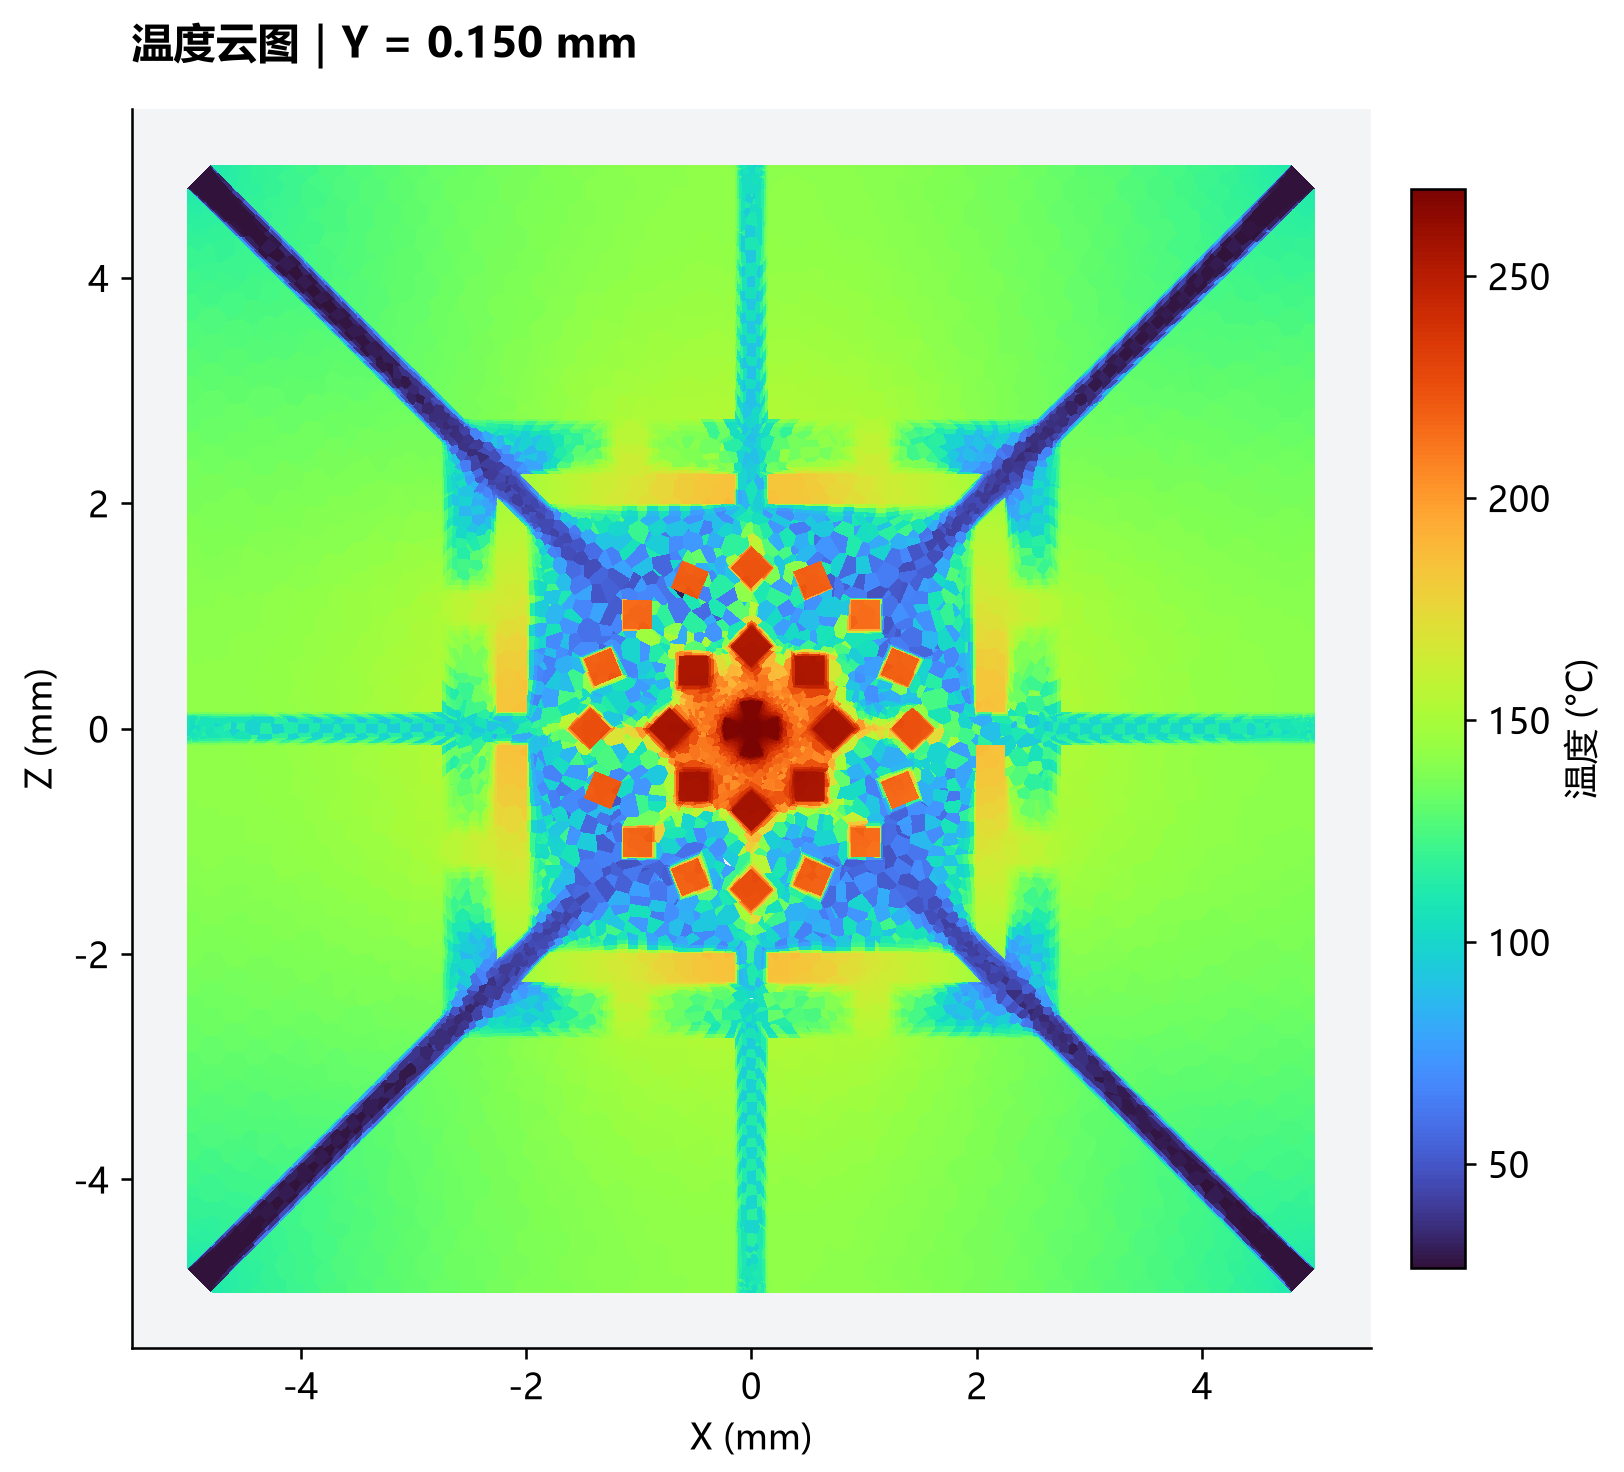
\includegraphics[width=\linewidth]{../../figs/01_temperature_midplane.png}
			\caption{方形微通道温度}
			\label{fig:repro-t}
		\end{subfigure}\hfill
		\begin{subfigure}{0.235\textwidth}
			\centering
			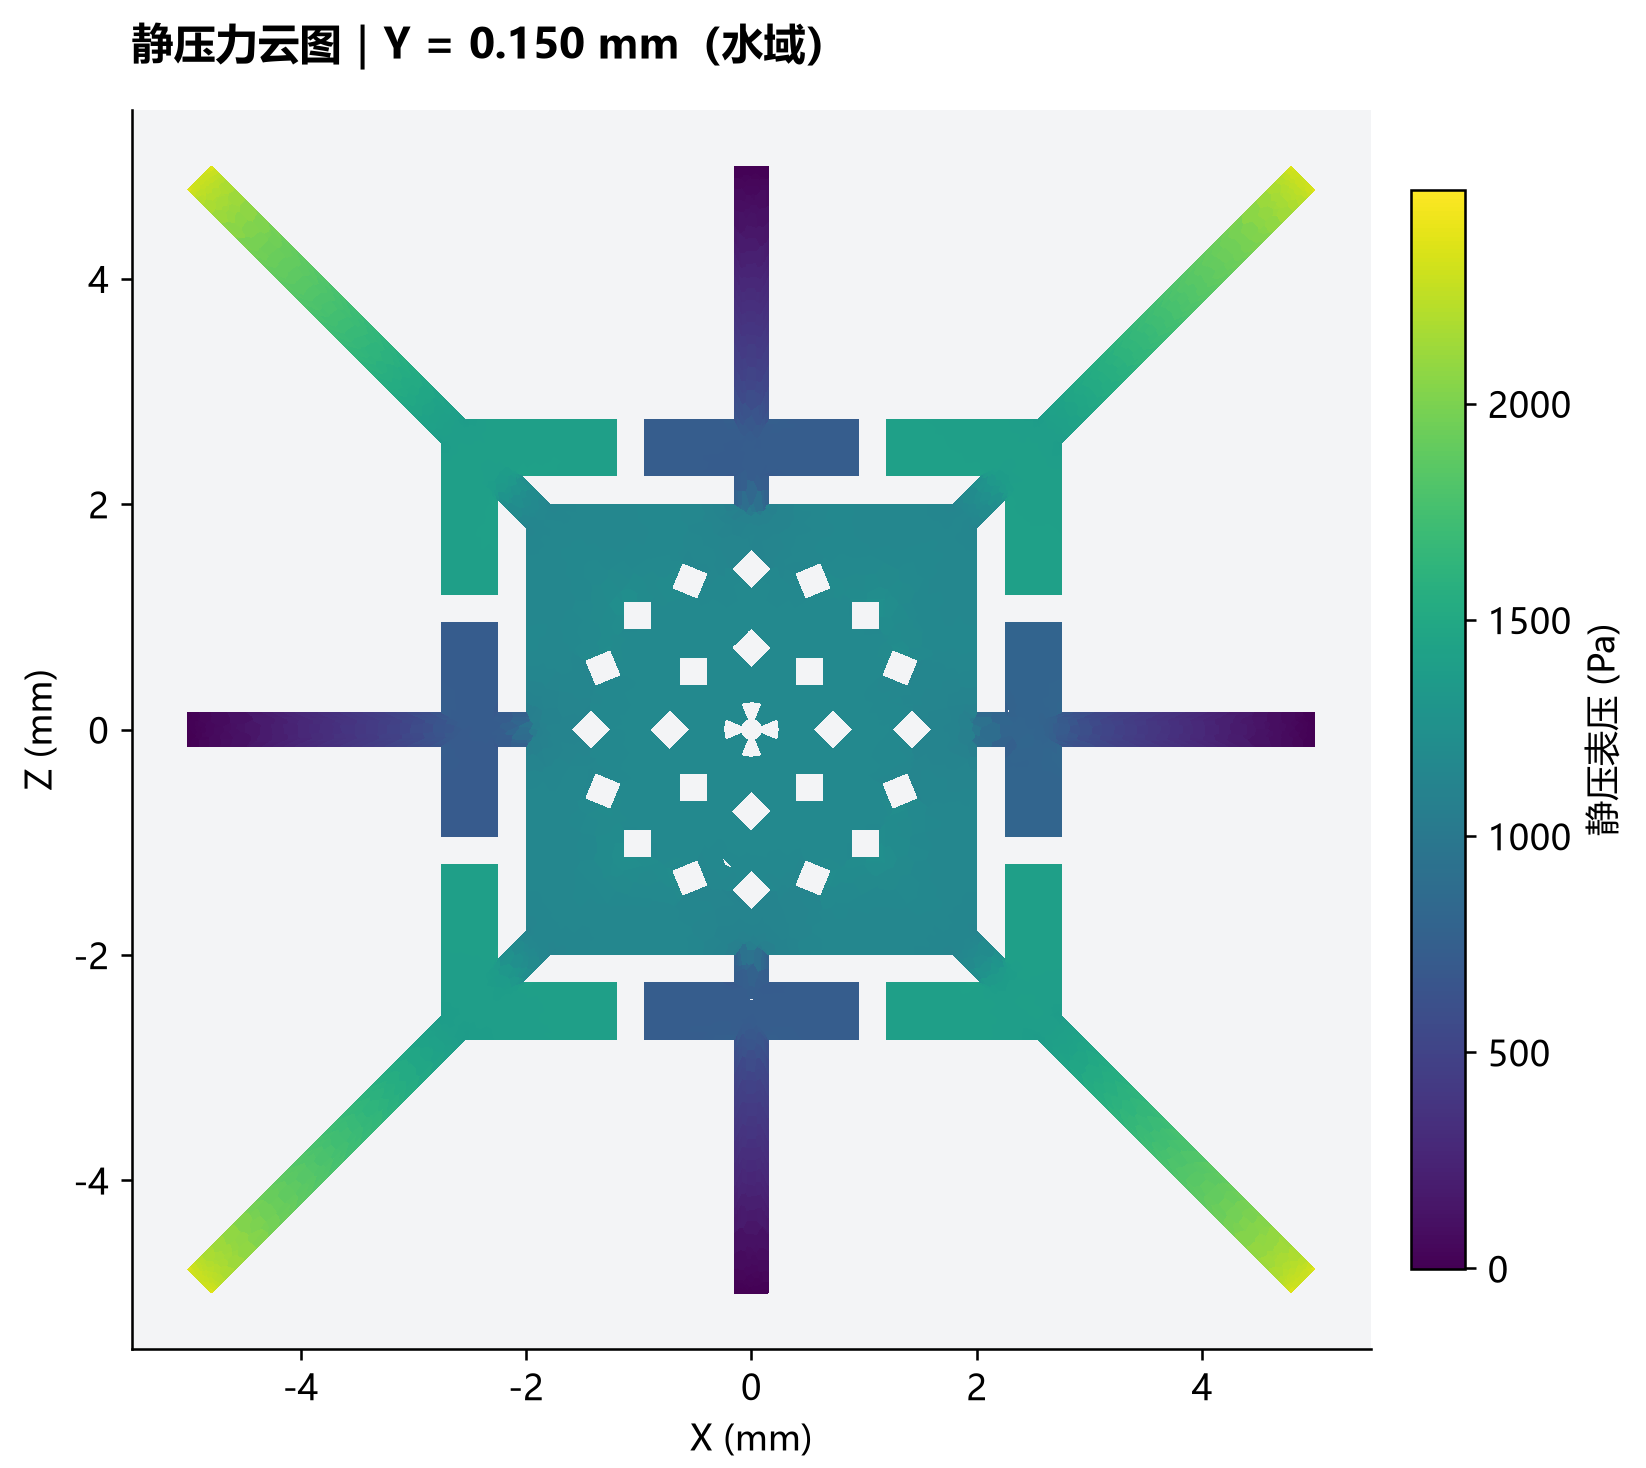
\includegraphics[width=\linewidth]{../../figs/02_pressure_midplane.png}
			\caption{方形微通道静压}
			\label{fig:repro-p}
		\end{subfigure}\hfill
		\begin{subfigure}{0.235\textwidth}
			\centering
			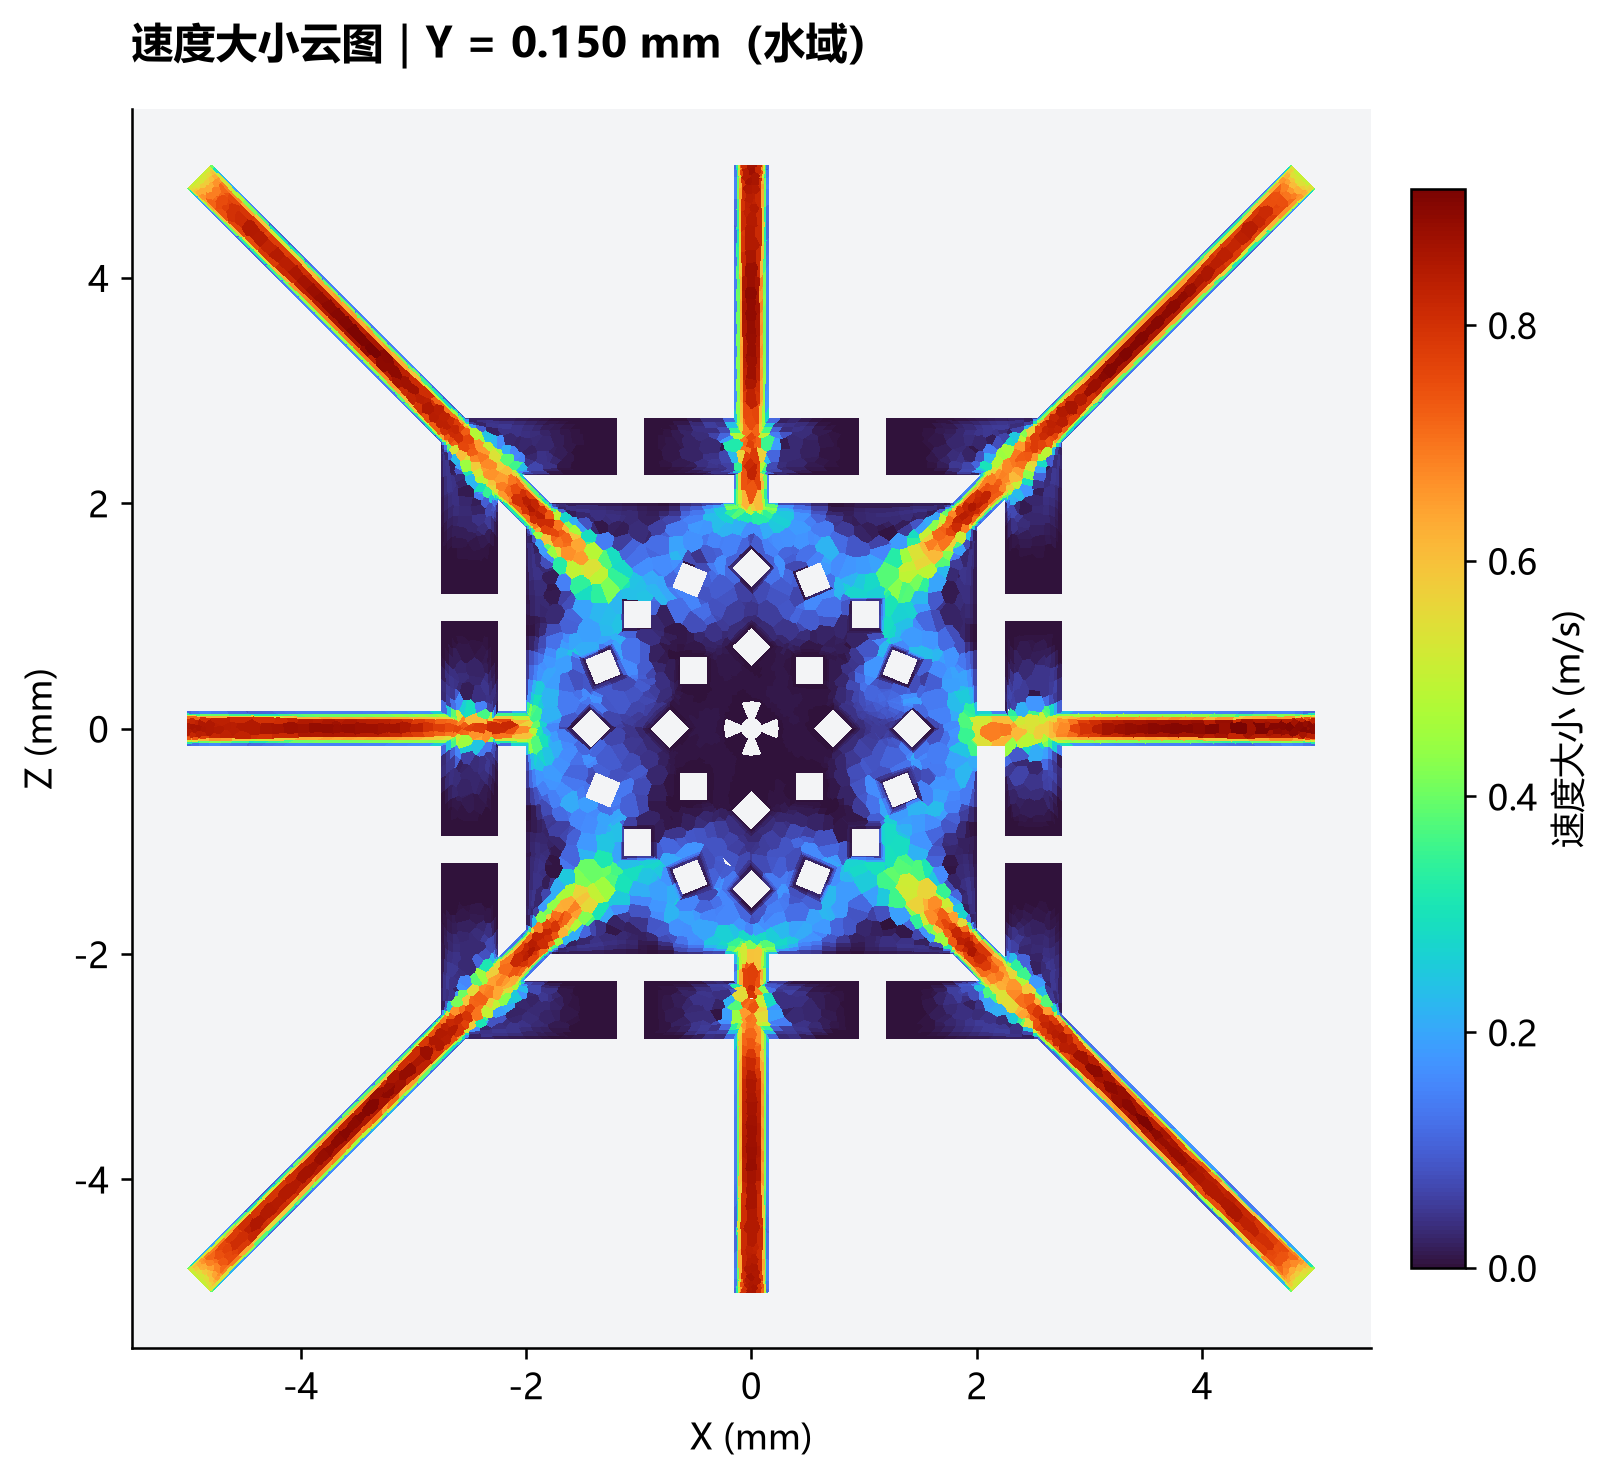
\includegraphics[width=\linewidth]{../../figs/03_speed_midplane.png}
			\caption{方形微通道速度大小}
			\label{fig:repro-v}
		\end{subfigure}\hfill
		\begin{subfigure}{0.235\textwidth}
			\centering
			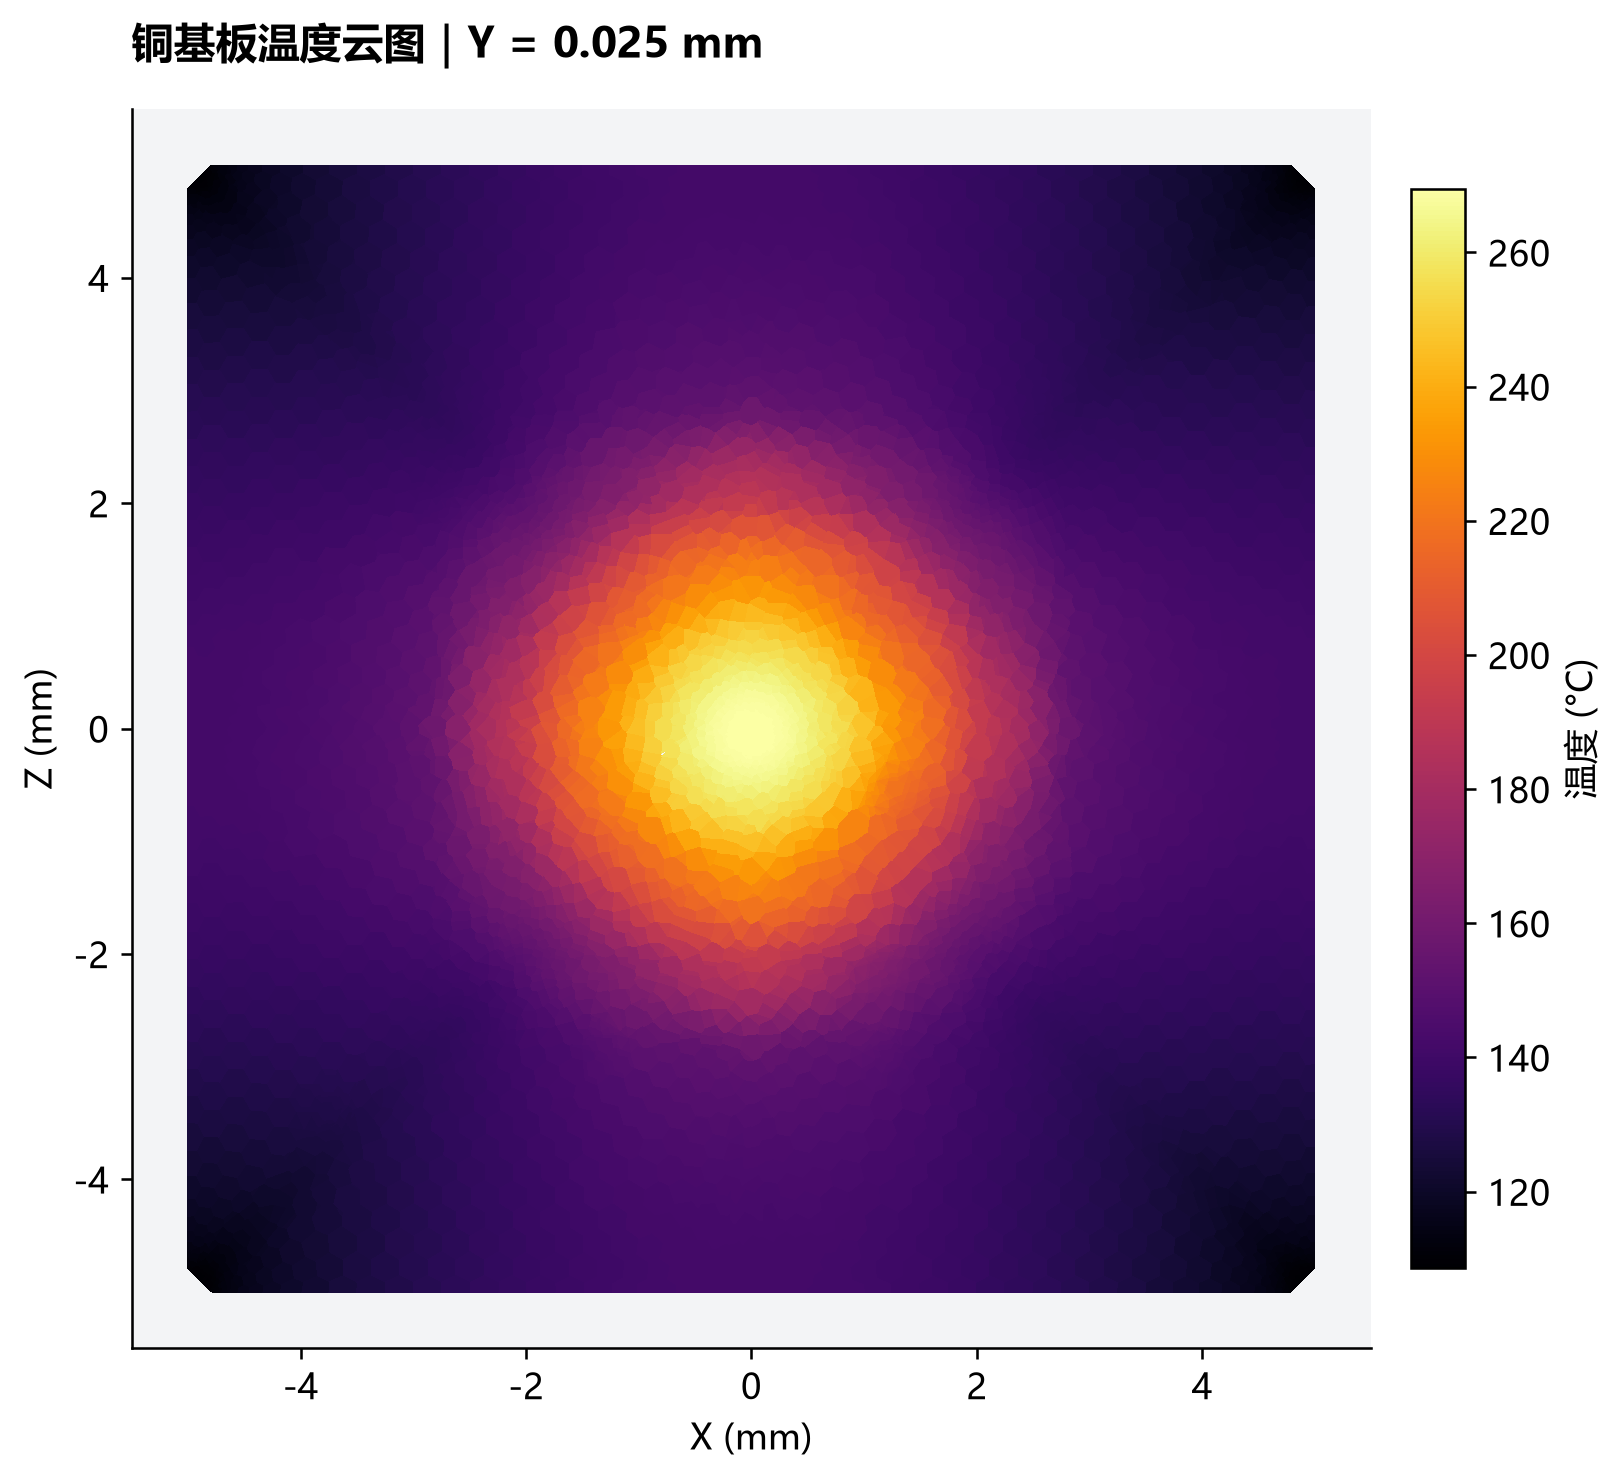
\includegraphics[width=\linewidth]{../../figs/04_copper_base_temperature.png}
			\caption{方形微通道铜板温度}
			\label{fig:repro-cu}
		\end{subfigure}

		\vspace{4pt}

		\begin{subfigure}{0.235\textwidth}
			\centering
			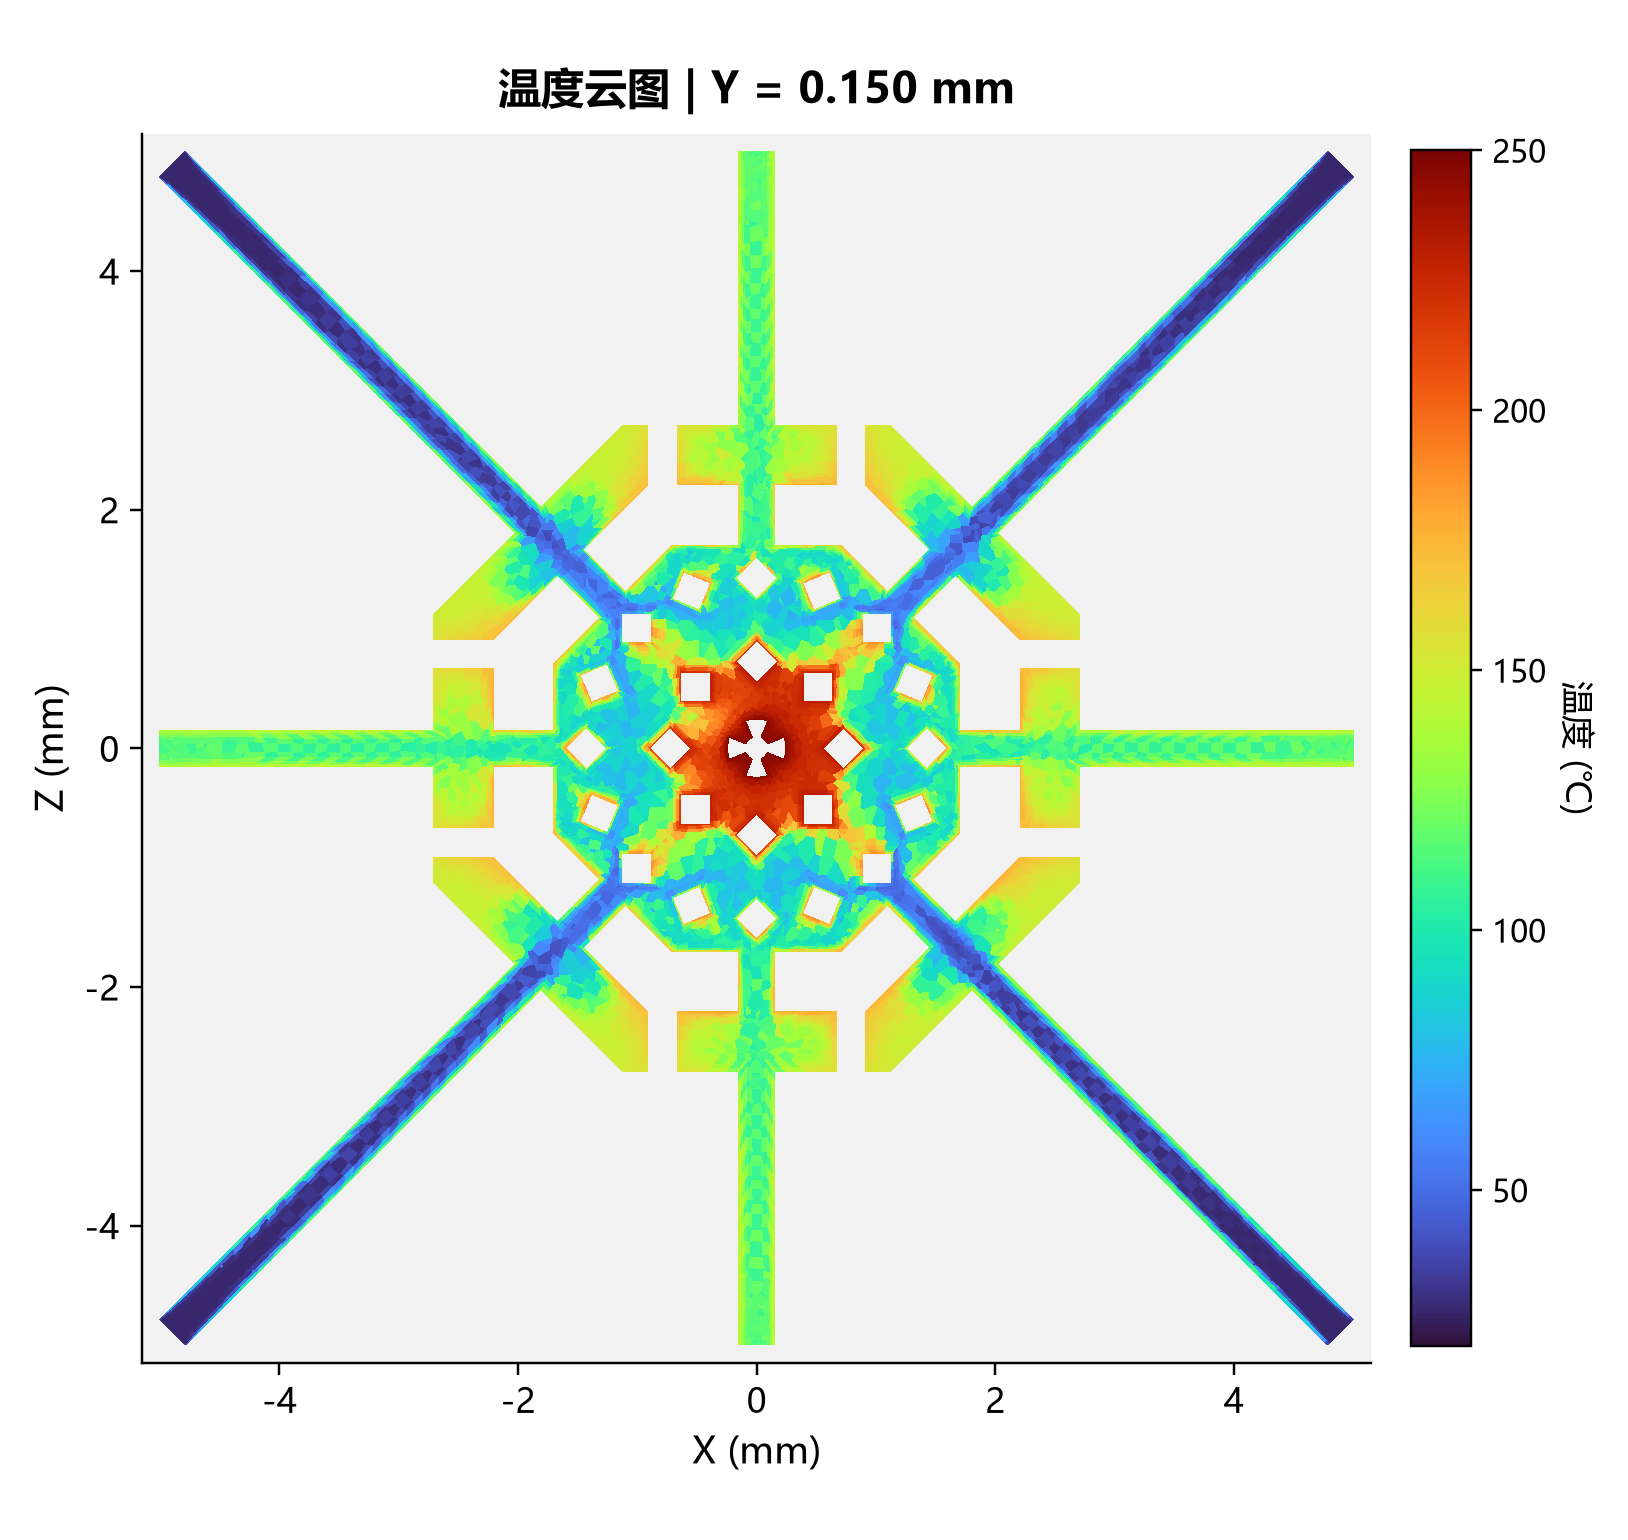
\includegraphics[width=\linewidth]{../../figs/05_temperature_midplane.png}
			\caption{六边形微通道温度}
			\label{fig:h5-t}
		\end{subfigure}\hfill
		\begin{subfigure}{0.235\textwidth}
			\centering
			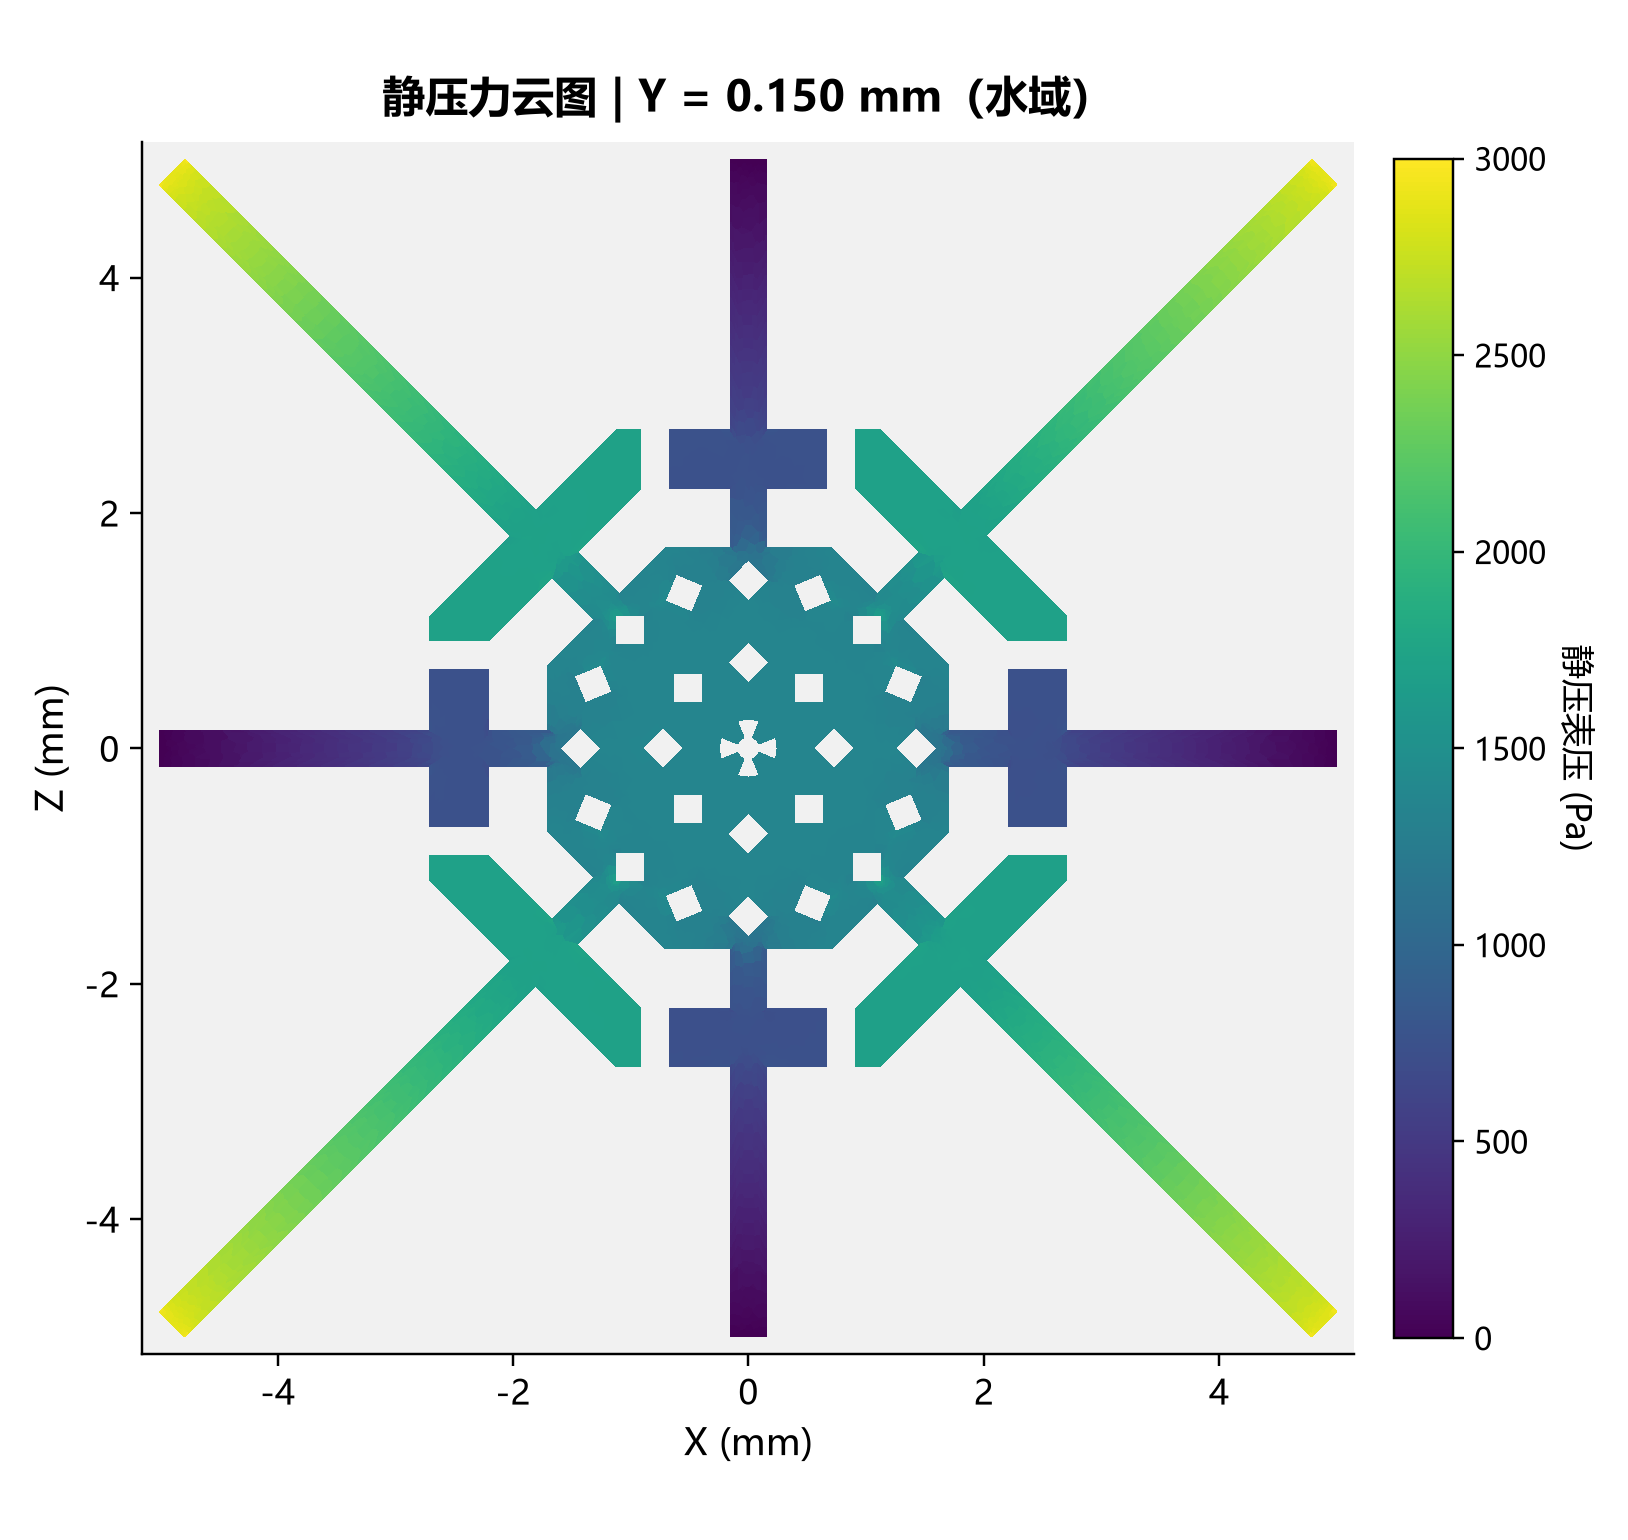
\includegraphics[width=\linewidth]{../../figs/06_pressure_midplane.png}
			\caption{六边形微通道静压}
			\label{fig:h5-p}
		\end{subfigure}\hfill
		\begin{subfigure}{0.235\textwidth}
			\centering
			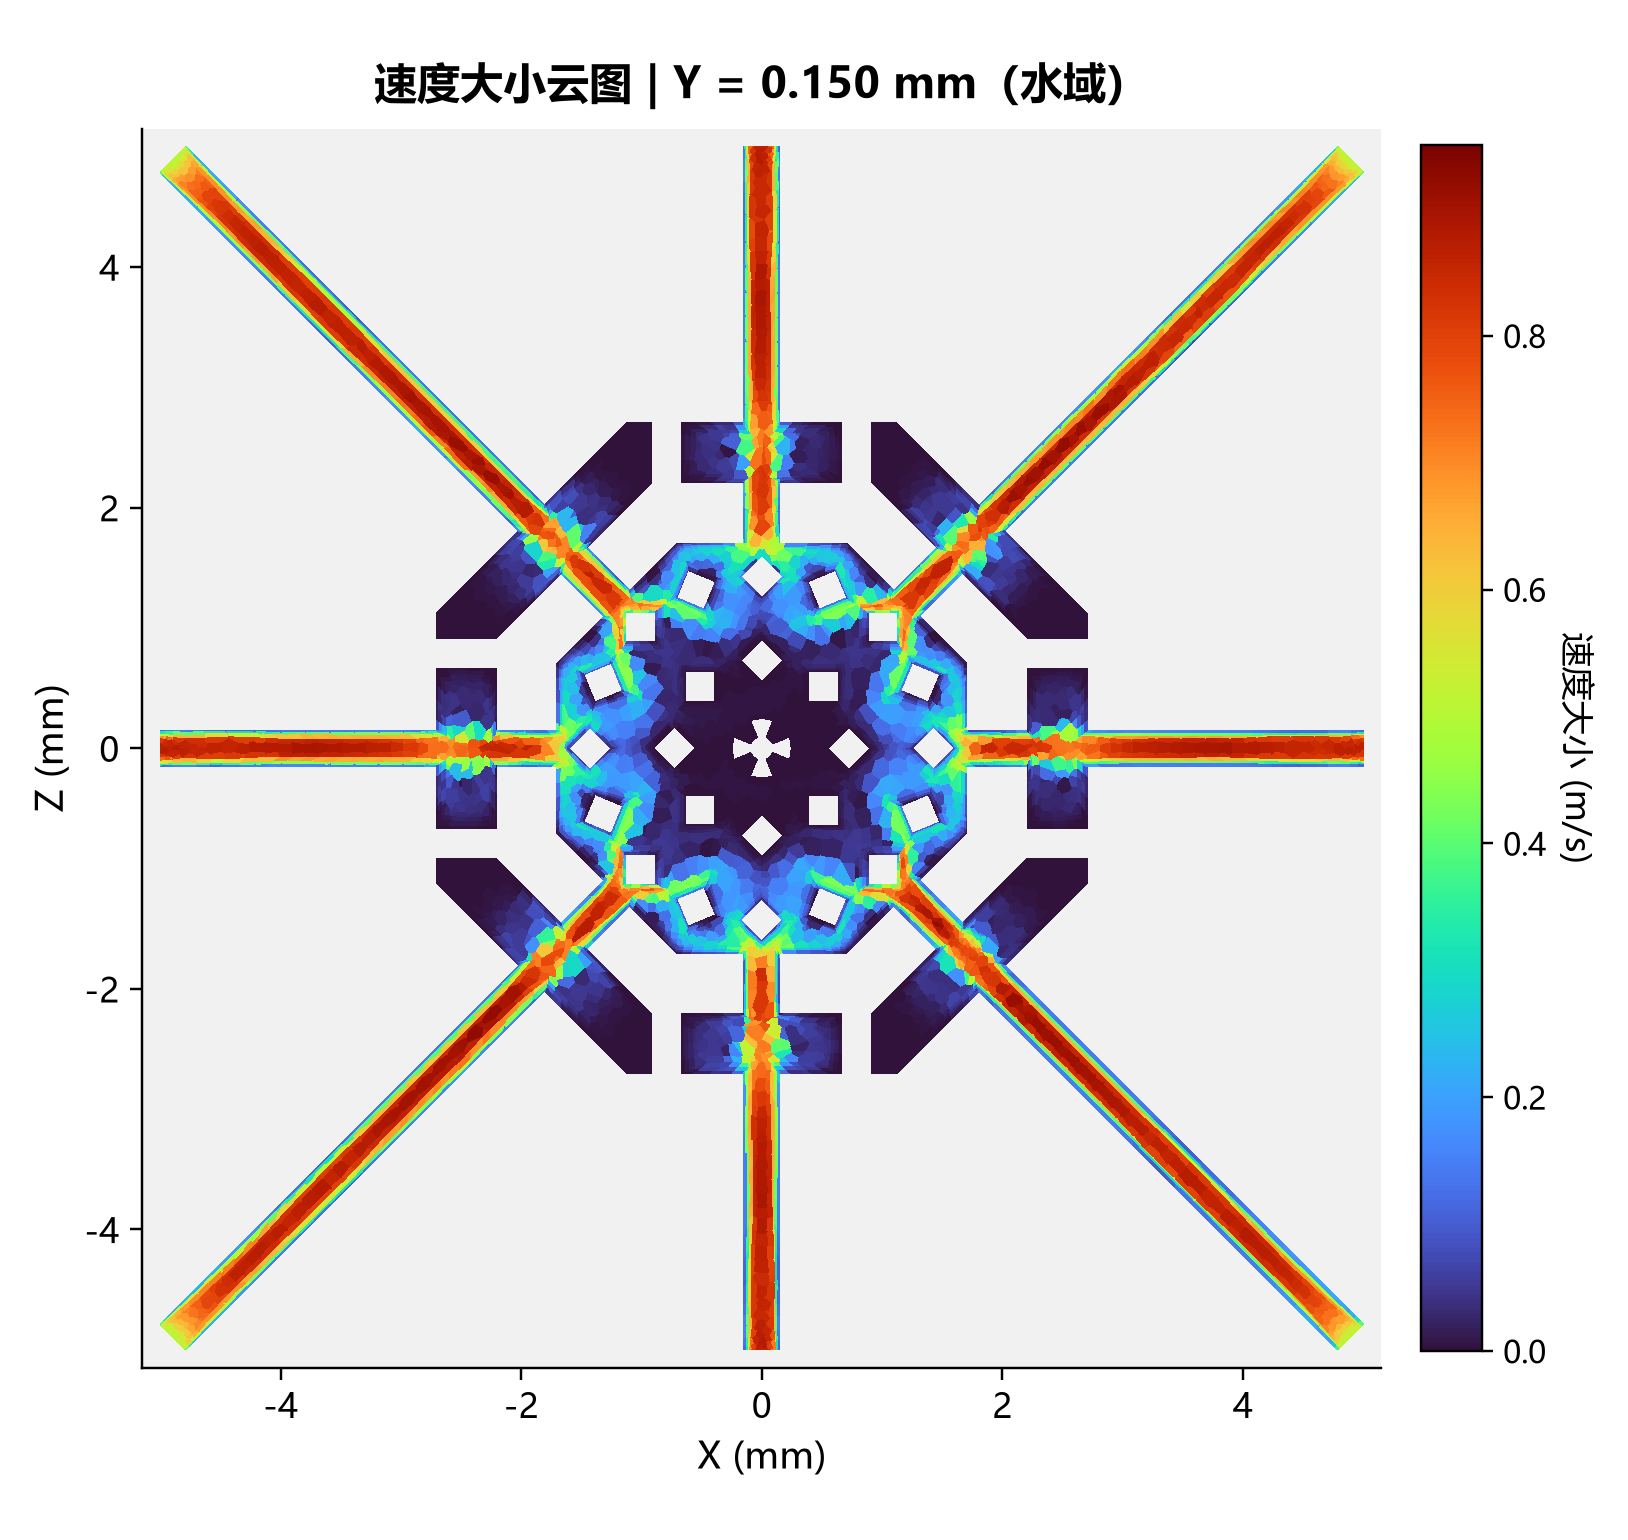
\includegraphics[width=\linewidth]{../../figs/07_speed_midplane.png}
			\caption{六边形微通道速度大小}
			\label{fig:h5-v}
		\end{subfigure}\hfill
		\begin{subfigure}{0.235\textwidth}
			\centering
			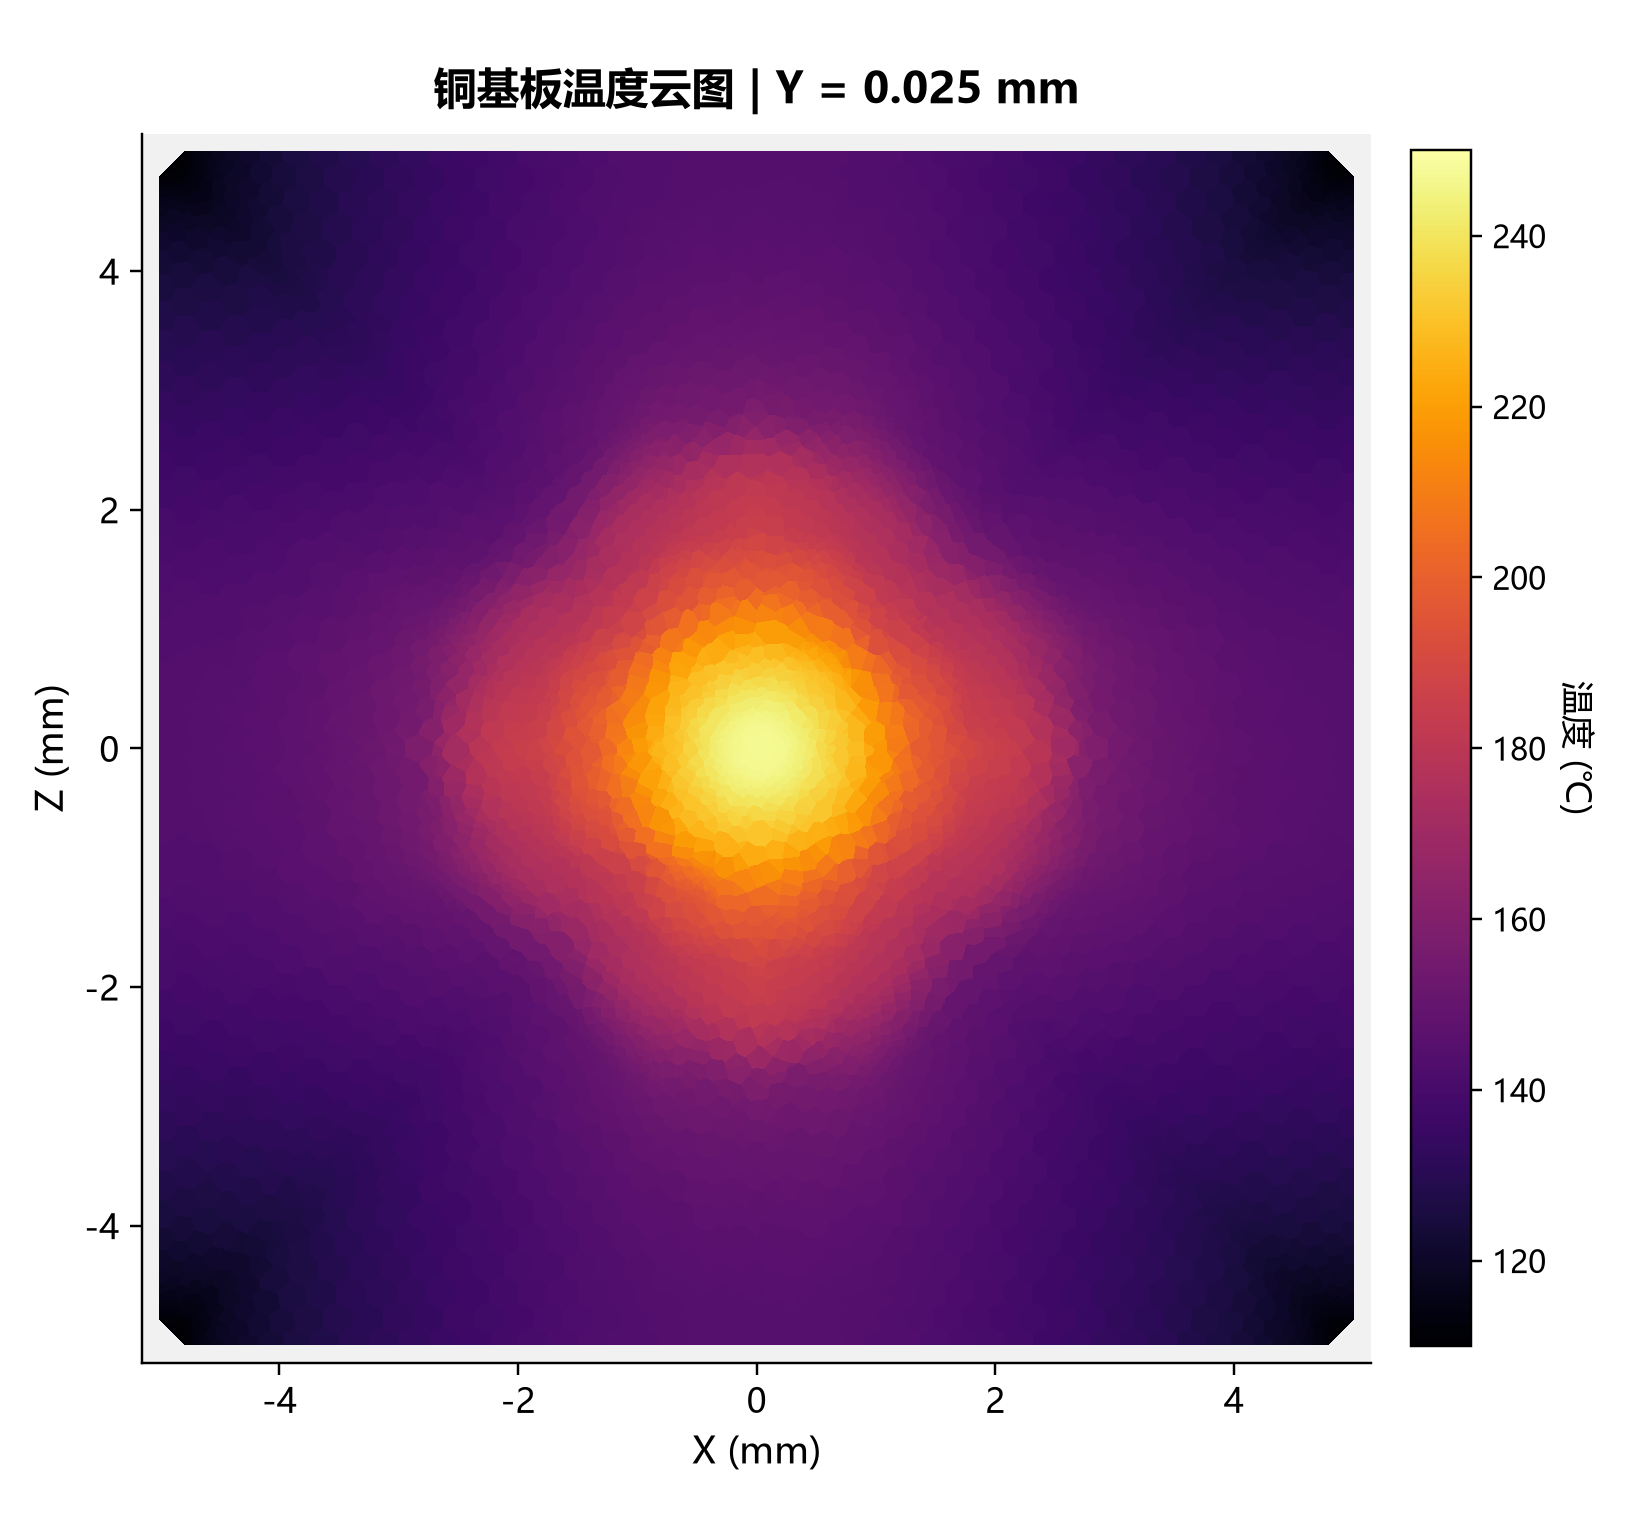
\includegraphics[width=\linewidth]{../../figs/08_copper_base_temperature.png}
			\caption{六边形微通道铜板温度}
			\label{fig:h5-cu}
		\end{subfigure}

		\vspace{4pt}

		\begin{subfigure}{0.235\textwidth}
			\centering
			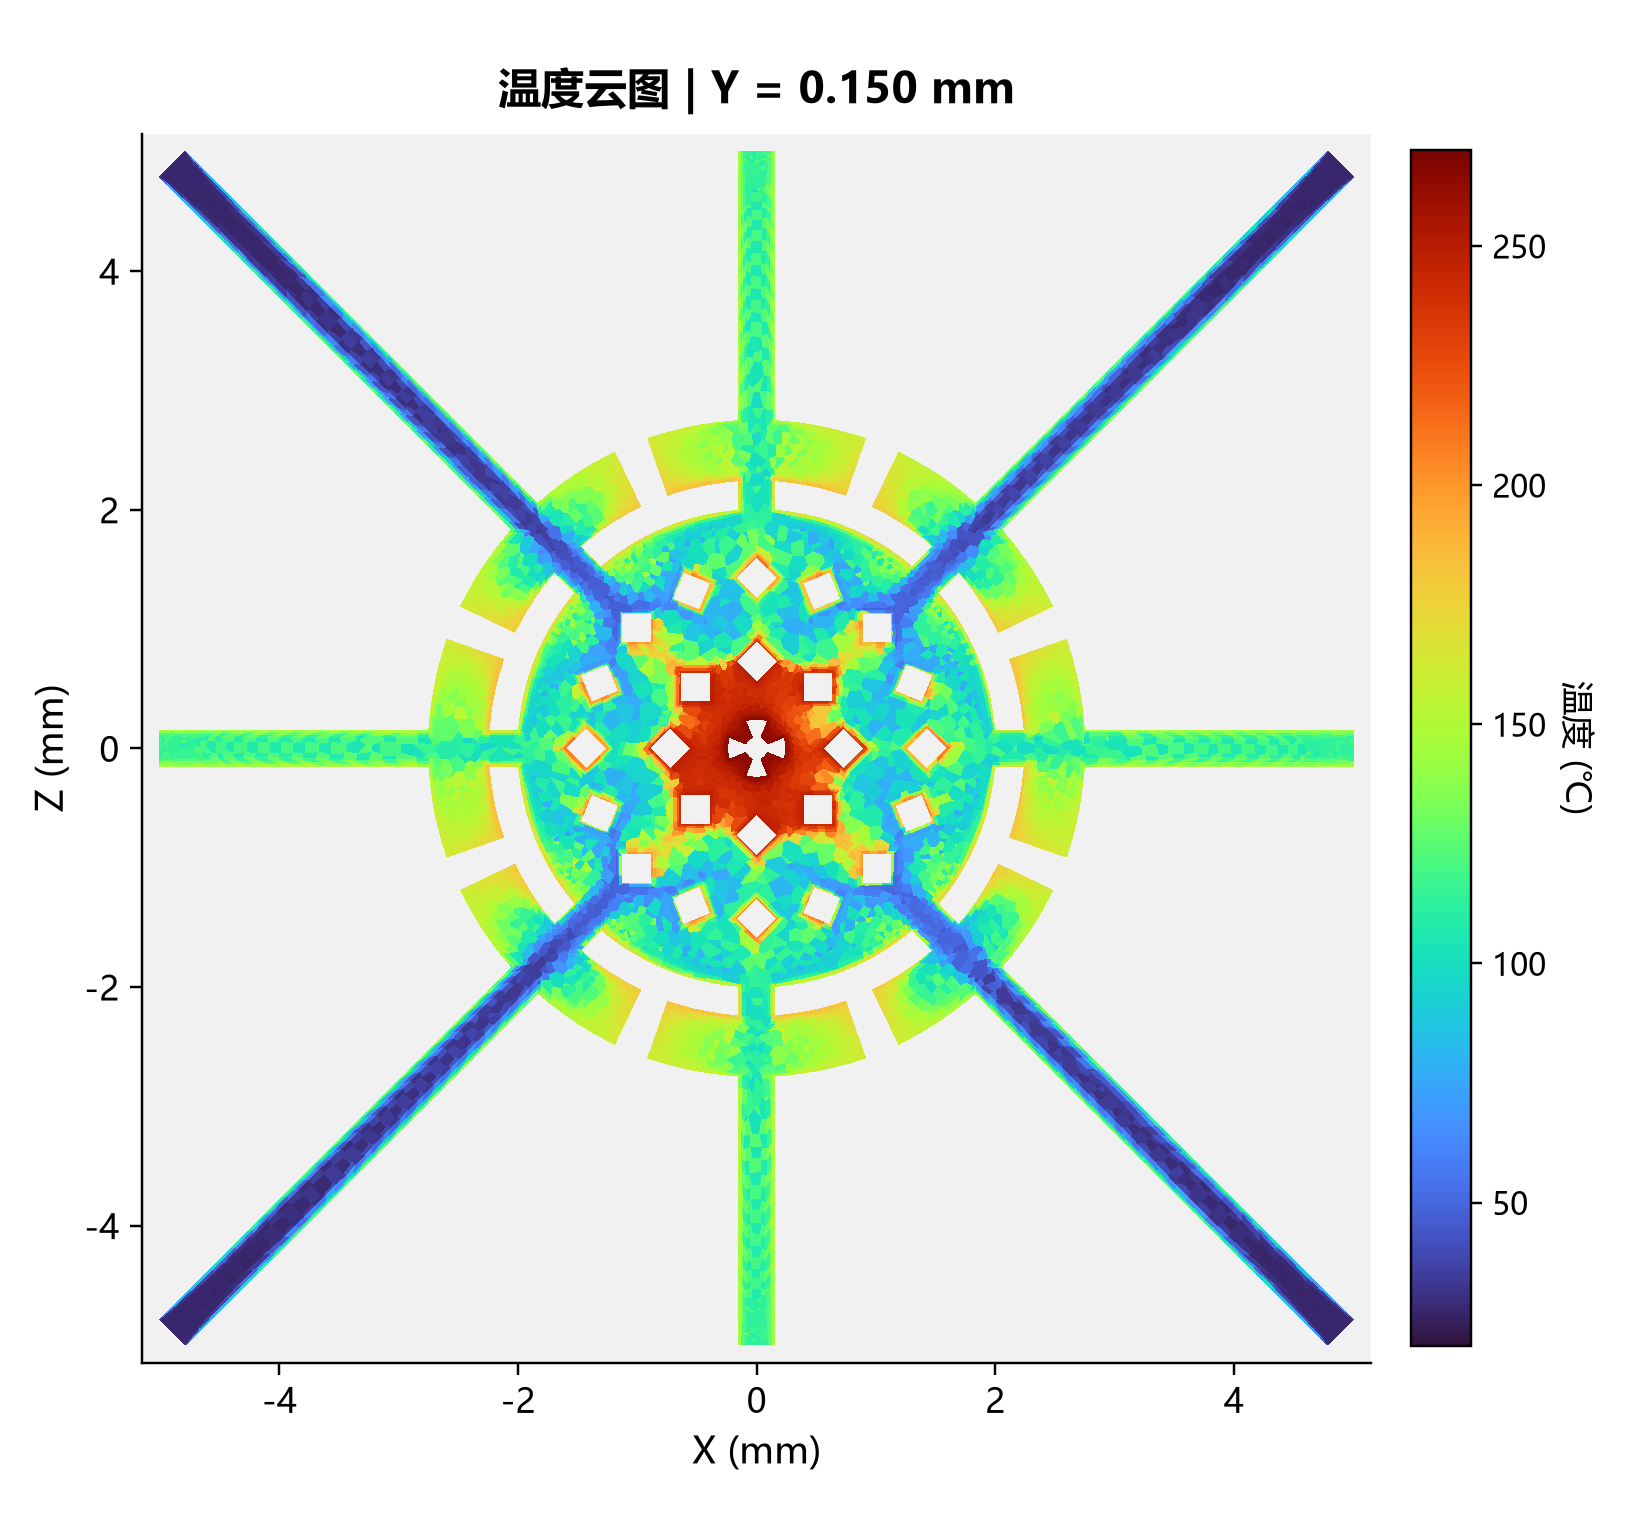
\includegraphics[width=\linewidth]{../../figs/09_temperature_midplane.png}
			\caption{圆形微通道温度}
			\label{fig:circle-t}
		\end{subfigure}\hfill
		\begin{subfigure}{0.235\textwidth}
			\centering
			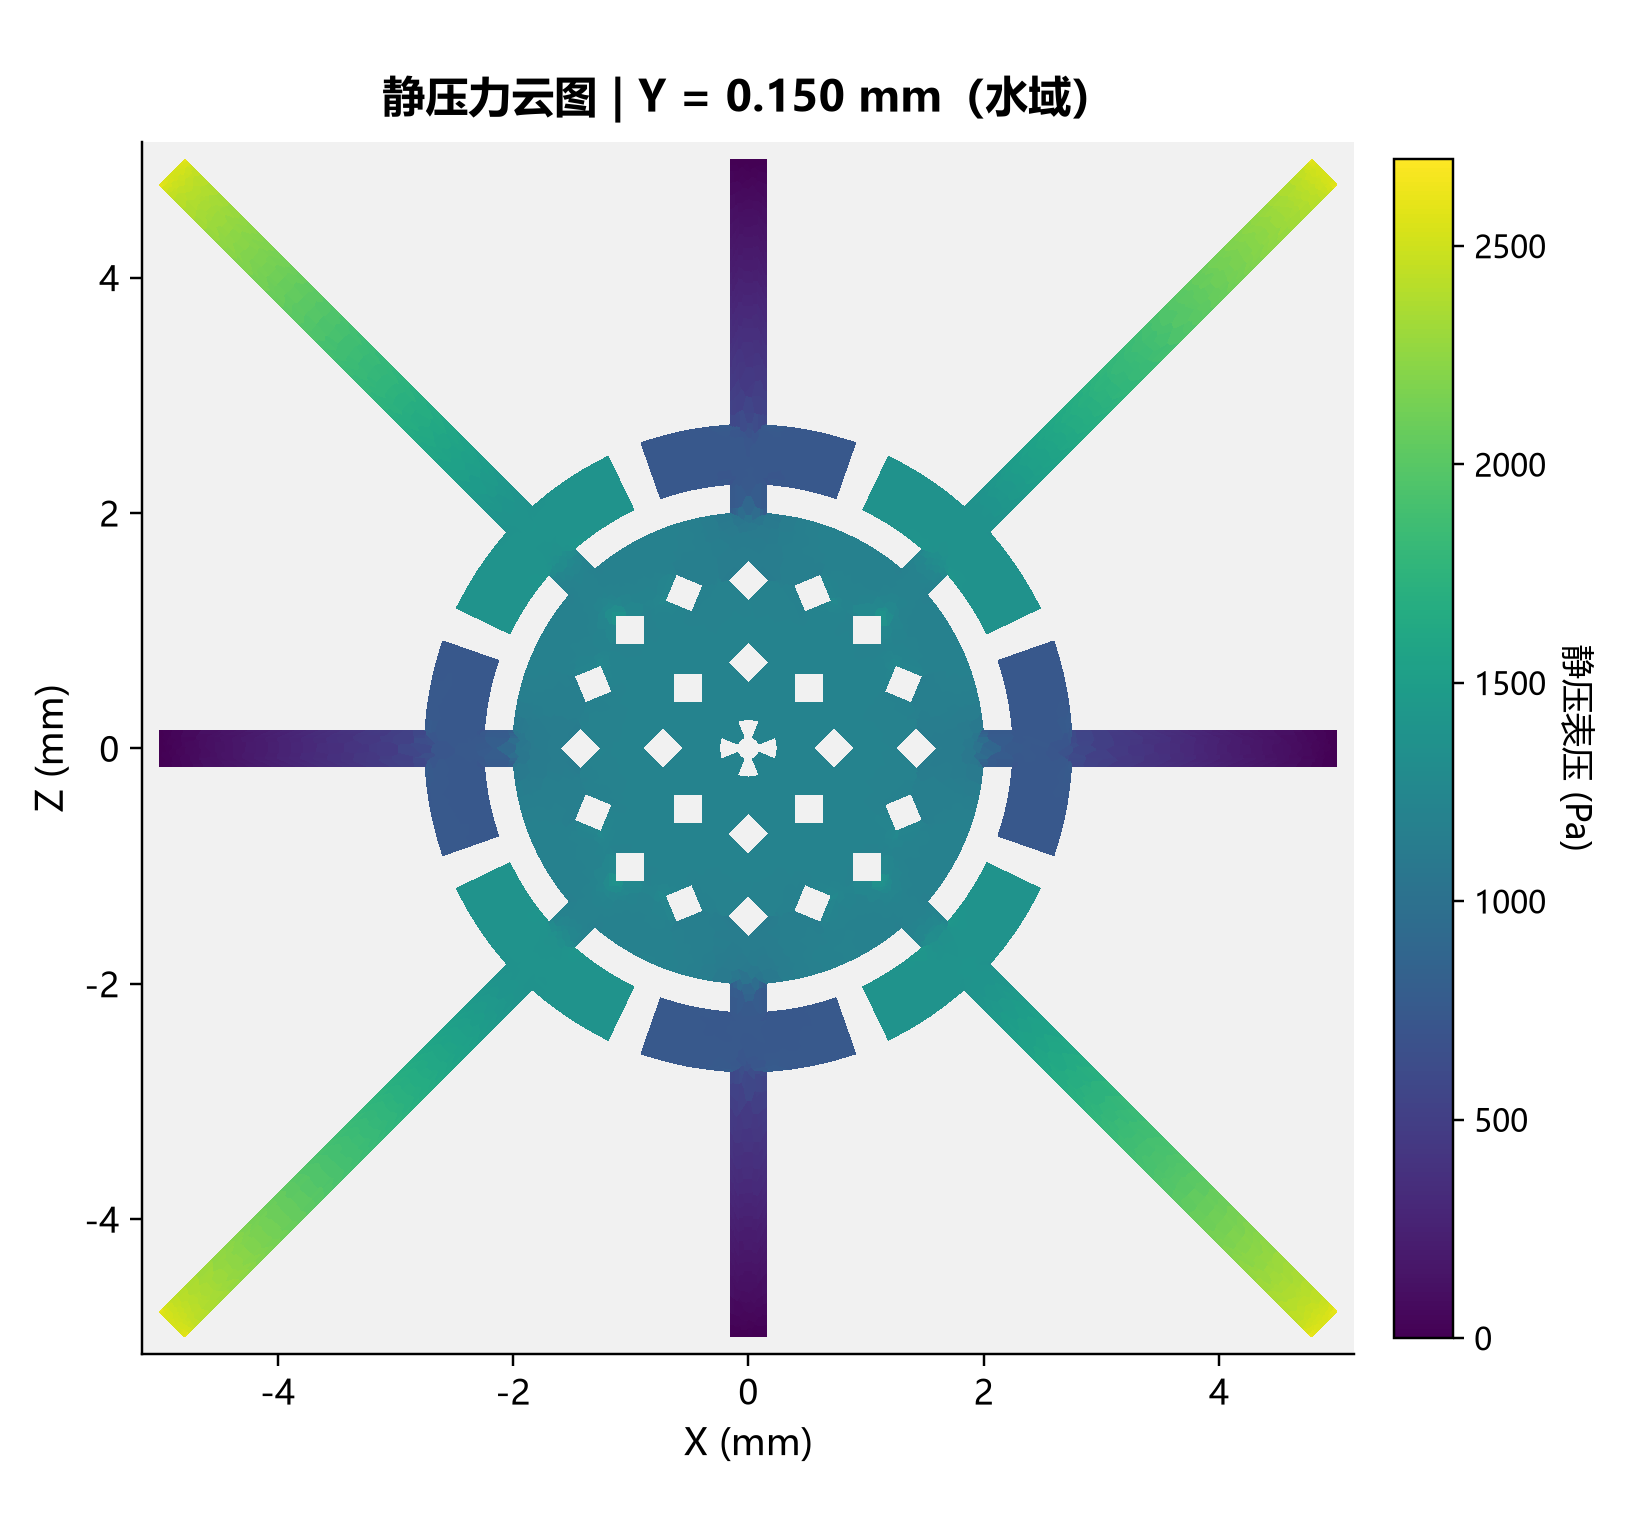
\includegraphics[width=\linewidth]{../../figs/10_pressure_midplane.png}
			\caption{圆形微通道静压}
			\label{fig:circle-p}
		\end{subfigure}\hfill
		\begin{subfigure}{0.235\textwidth}
			\centering
			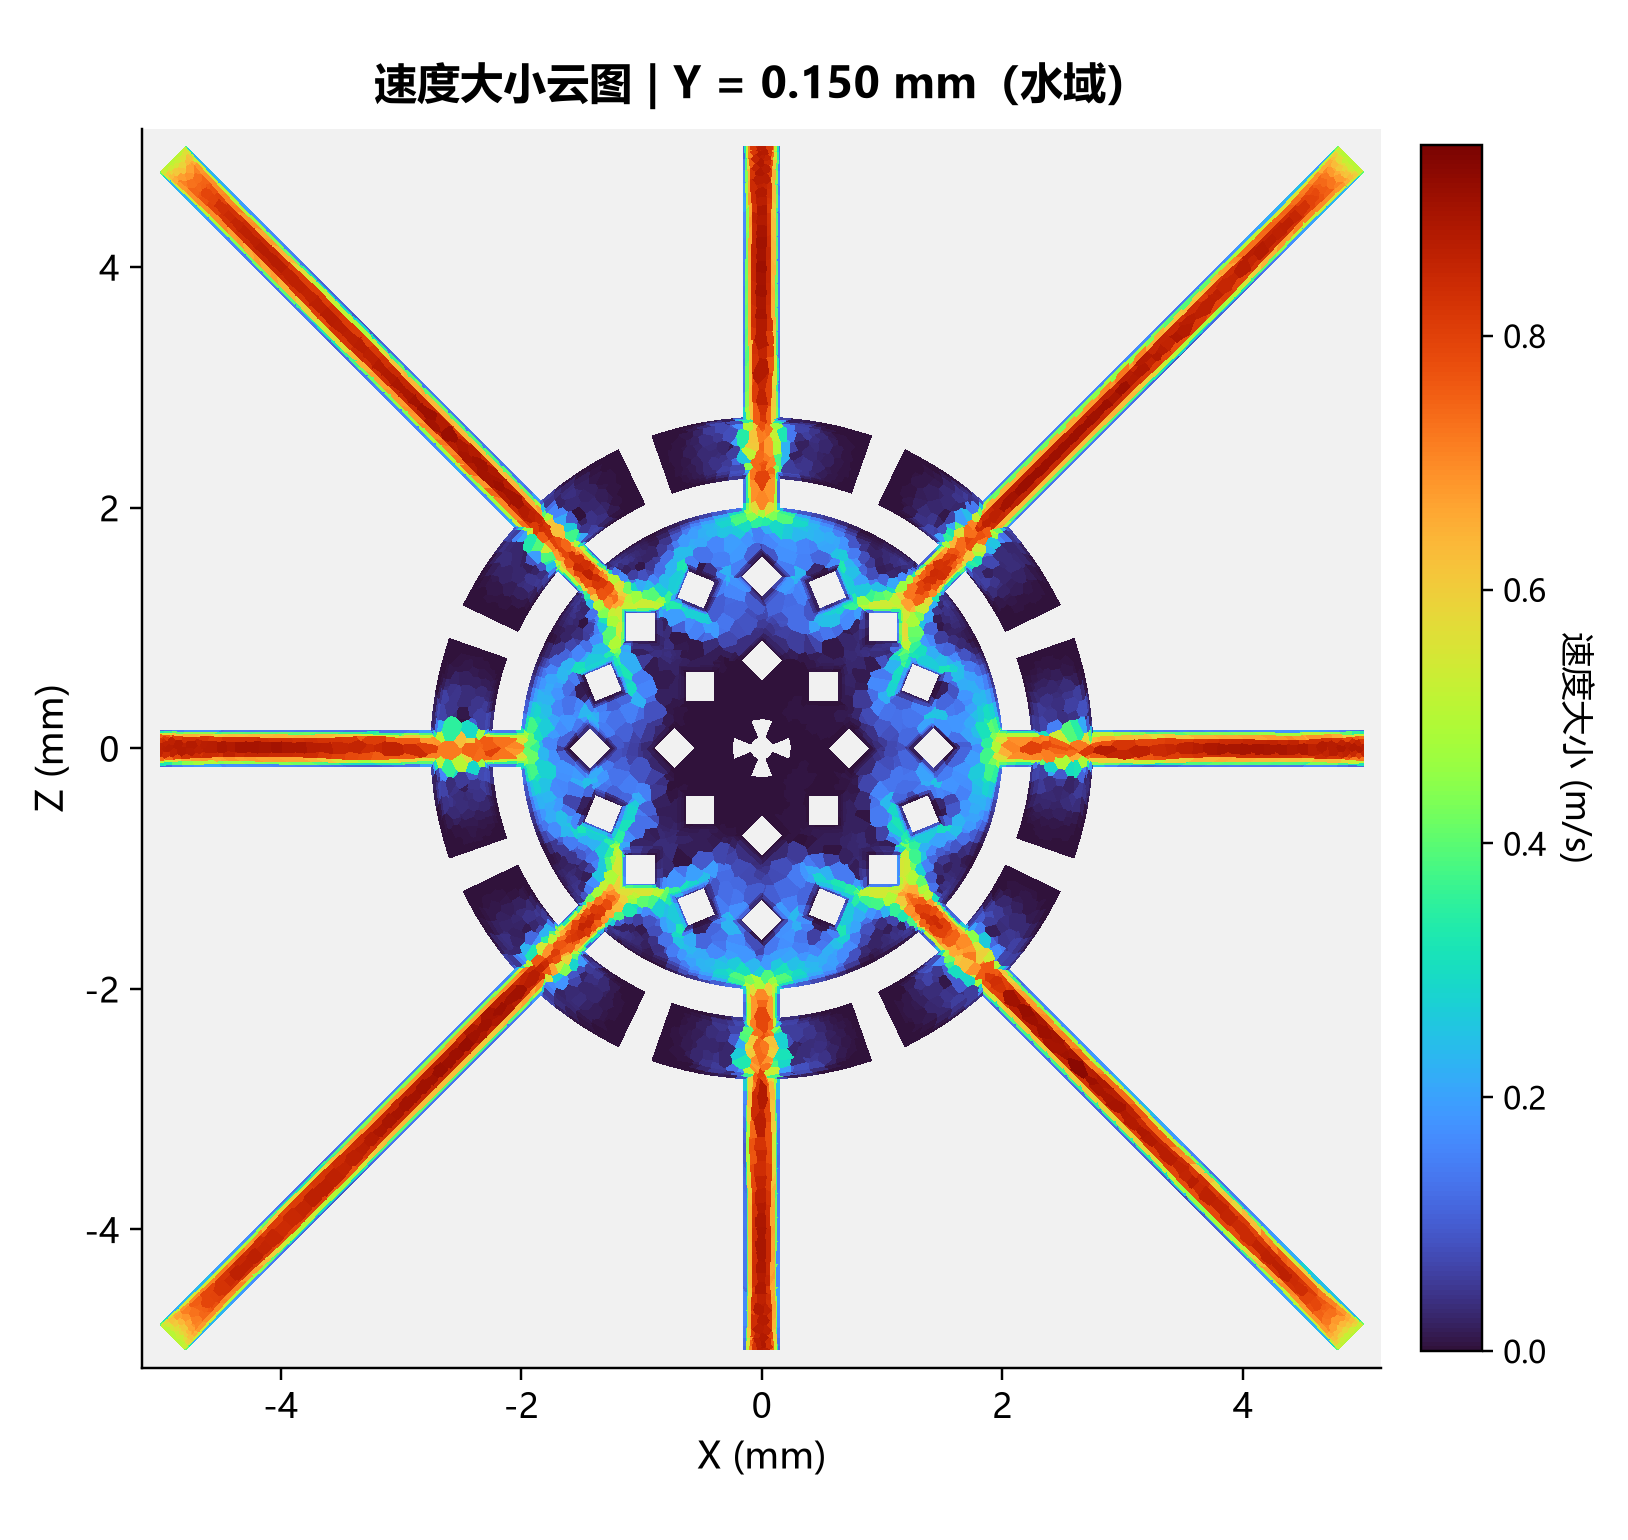
\includegraphics[width=\linewidth]{../../figs/11_speed_midplane.png}
			\caption{圆形微通道速度大小}
			\label{fig:circle-v}
		\end{subfigure}\hfill
		\begin{subfigure}{0.235\textwidth}
			\centering
			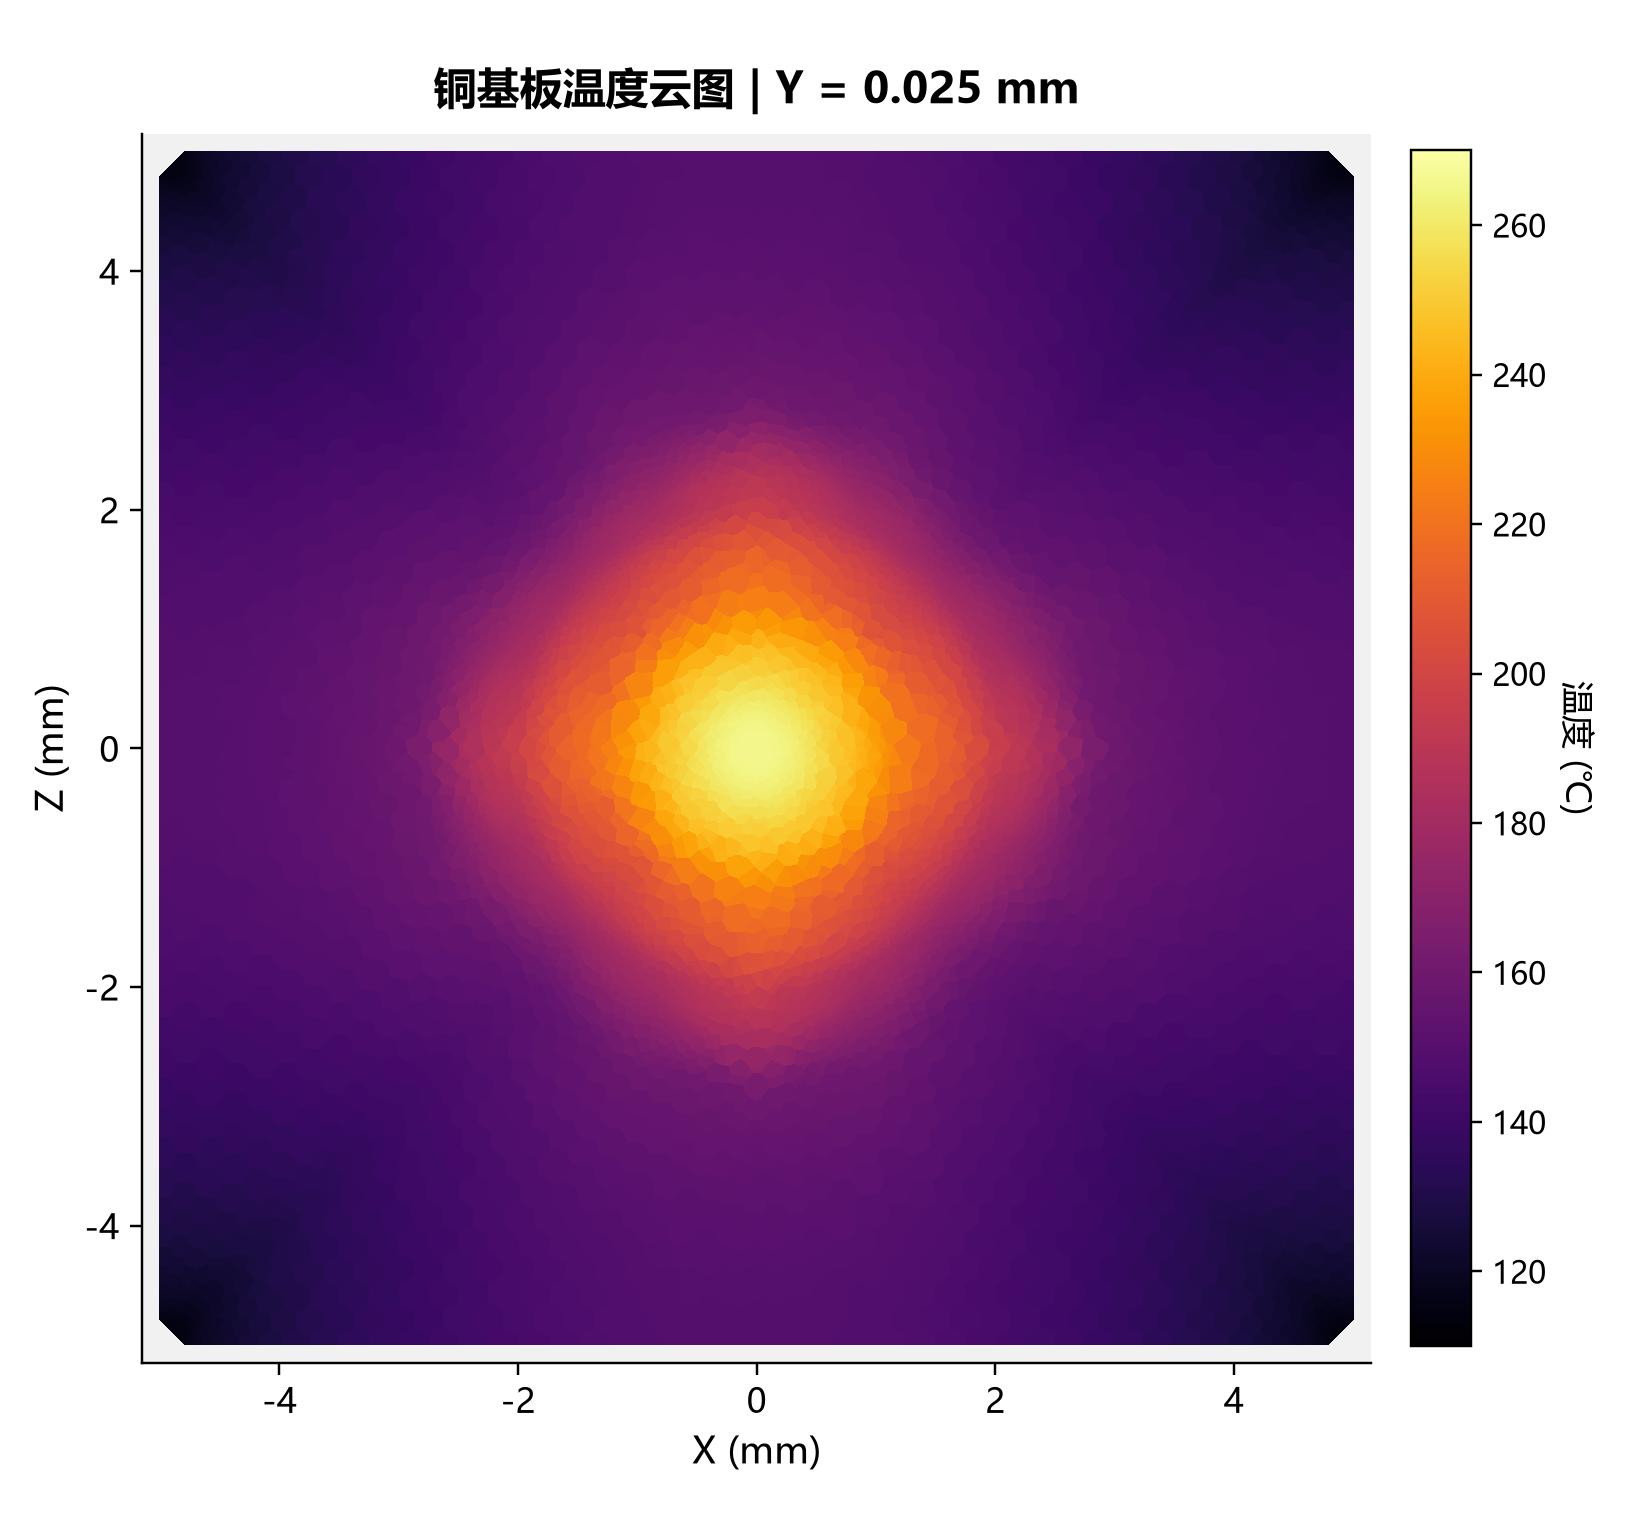
\includegraphics[width=\linewidth]{../../figs/12_copper_base_temperature.png}
			\caption{圆形微通道铜板温度}
			\label{fig:circle-cu}
		\end{subfigure}
		\caption{复现算例的后处理云图： (a)--(l) 为流道的参考结果。三行均依次为水侧 $Y=0.150$ mm 中截面的温度、静压（表压）与速度大小，以及铜基板 $Y=0.025$ mm 截面的温度。灰白空区为截面外或固体遮罩}
		\label{fig:repro}
	\end{figure}
\clearpage
\setcounter{figure}{1}
\begin{figure}[H]
		\centering
		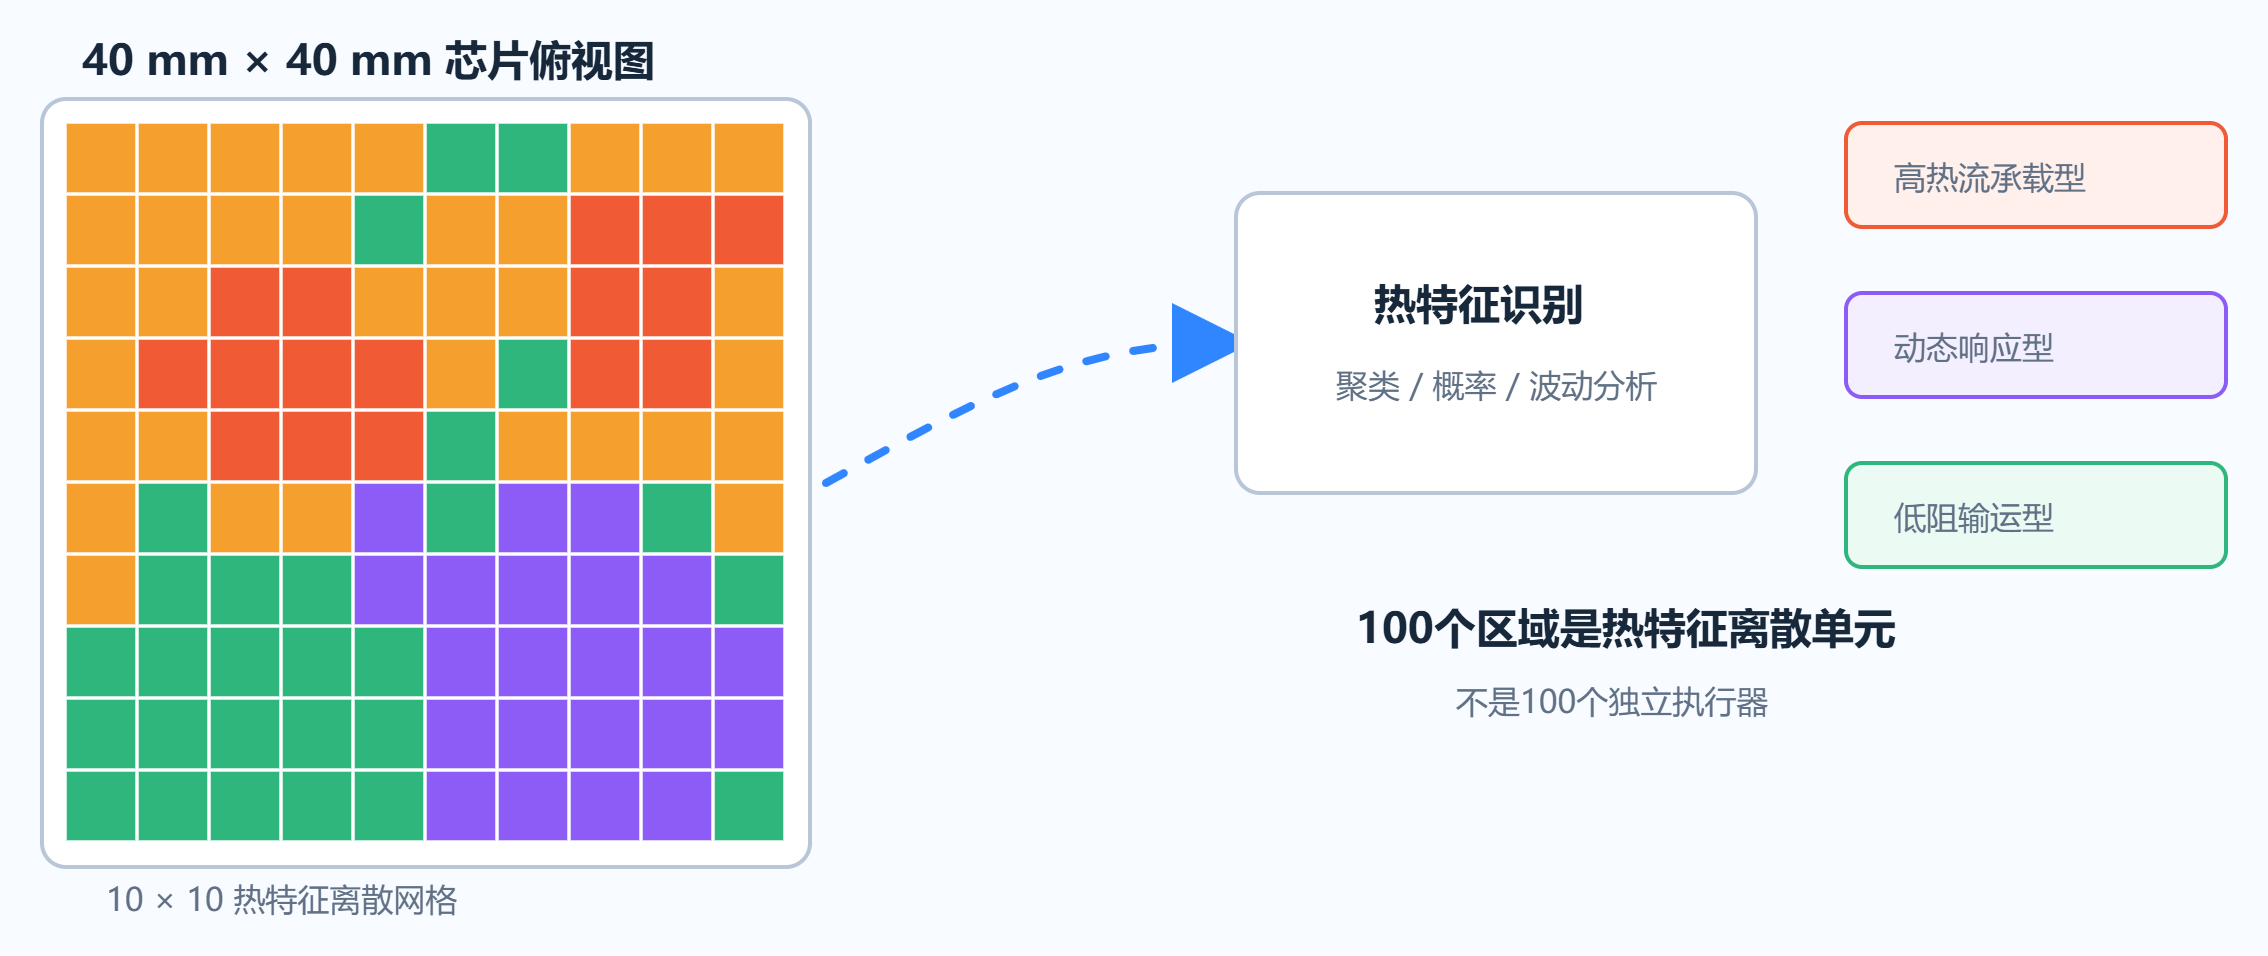
\includegraphics[width=0.94\linewidth]{../../figs/month1_小块热特征分类.png}
		\caption{小块热特征分类：$40\,\mathrm{mm}\times40\,\mathrm{mm}$ 芯片按 $10\times10$ 离散为 100 个区域，经聚类、概率与波动分析归为高热流承载型、动态响应型与低阻输运型。100 个区域是热特征离散单元，不是 100 个独立执行器。}
		\label{fig:block-classify}
	\end{figure}
\clearpage
\setcounter{figure}{2}
\begin{figure}[H]
		\centering
		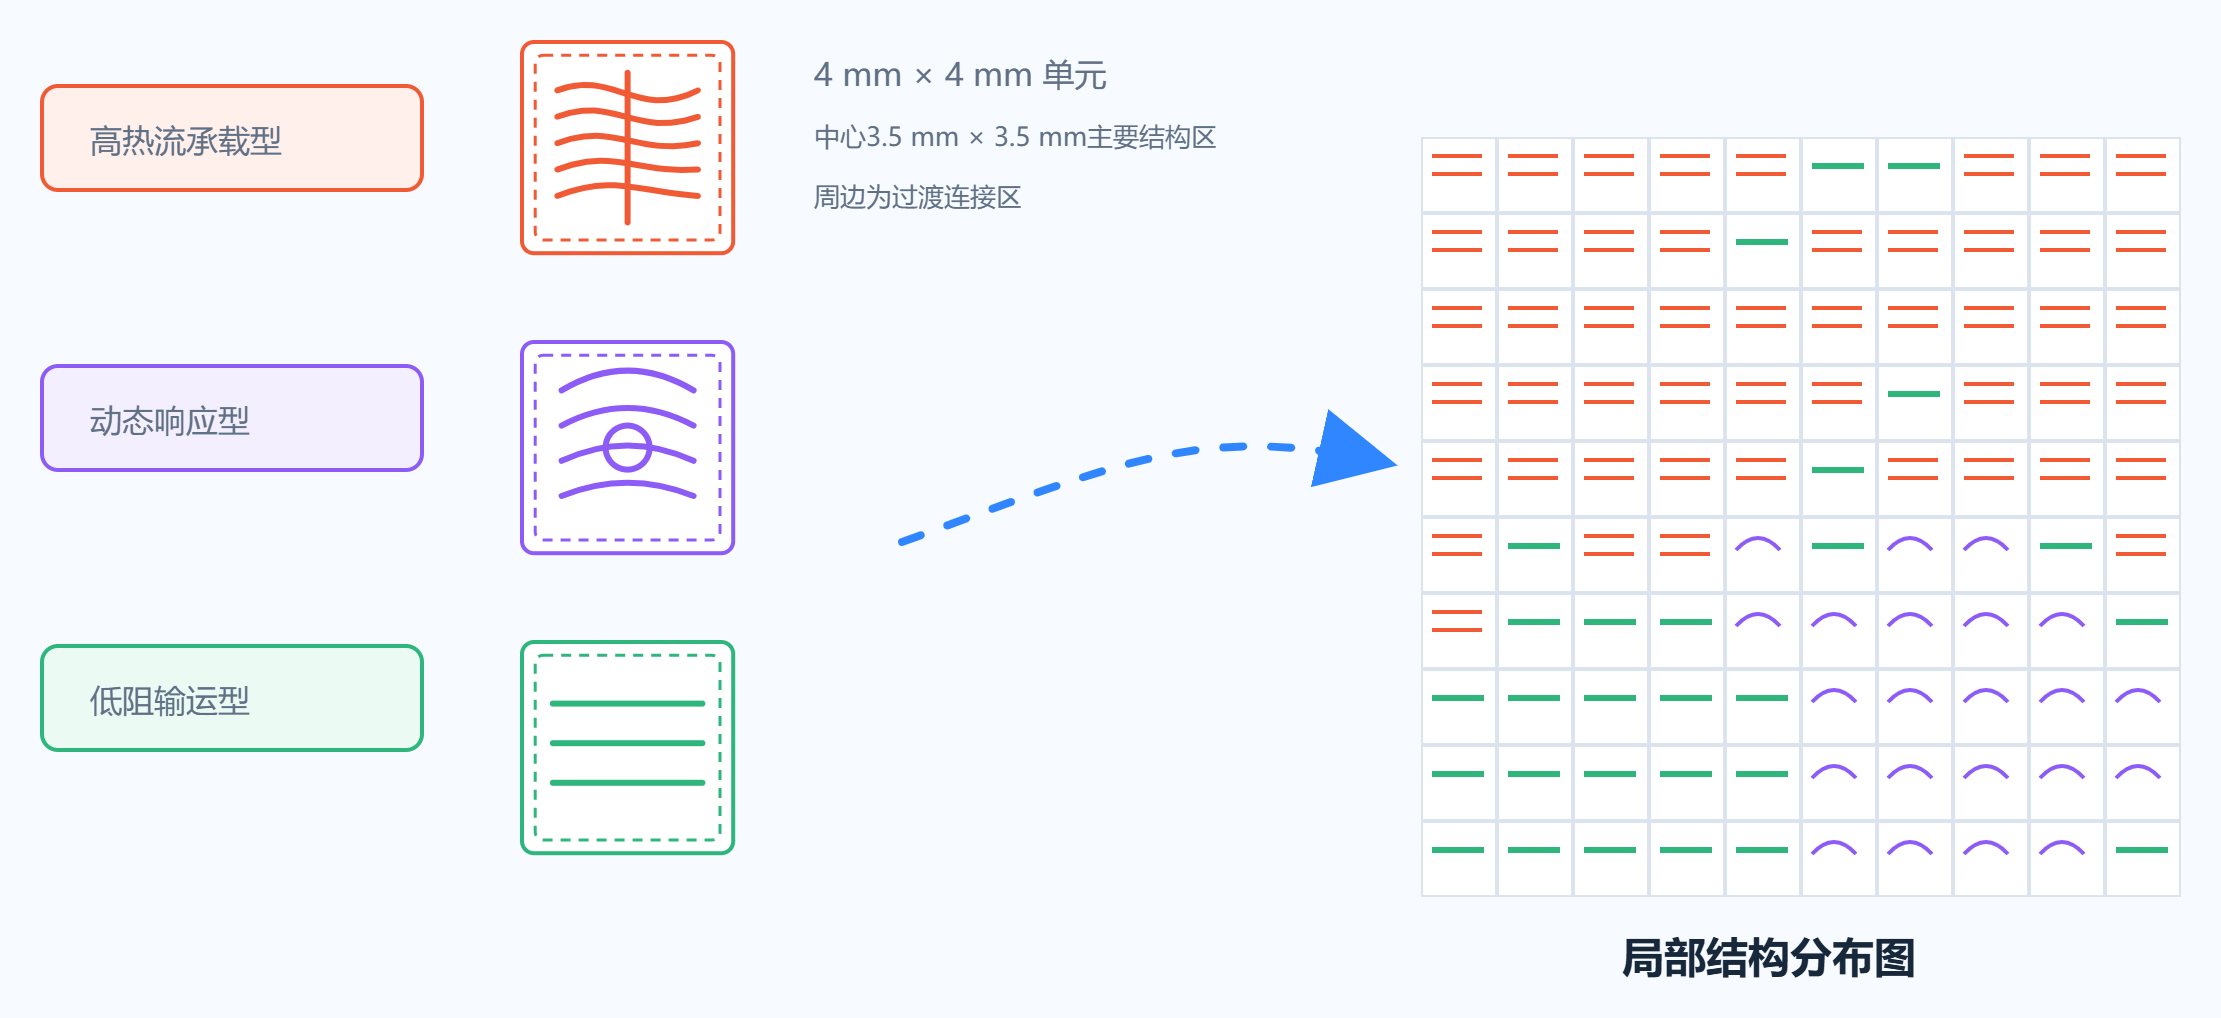
\includegraphics[width=0.94\linewidth]{../../figs/month1_局部微结构匹配.png}
		\caption{局部微结构匹配：每个 $4\,\mathrm{mm}\times4\,\mathrm{mm}$ 单元的中心 $3.5\,\mathrm{mm}\times3.5\,\mathrm{mm}$ 为主体结构区，周边为过渡连接区；高热流承载型对应扰流柱肋片，动态响应型对应仿生曲面，低阻输运型对应直通道，由此得到局部结构分布图。}
		\label{fig:block-match}
	\end{figure}
\clearpage
\setcounter{table}{3}
\begin{table}[H]\centering
\caption{本月工作与材料状态}\label{tab:tasks}
\begin{tabularx}{\textwidth}{@{}Y Y Y@{}}
\toprule
\rowcolor{ydzjlight} 工作 & 状态 & 依据或缺口 \\
\midrule
仿真软件学习与复现 & 已有材料 & 方形、圆形、六边形结构及后处理图 \\
初步小块理论 & 概念形成 & 来自文献与非均匀热负荷思考，适用分界线尚未建立 \\
物理与 UDF 学习 & 初步尝试 & 理解变物性、经验公式及接口，正式修改后移至月三 \\
自控基础学习 & 已有整理 & 一阶、二阶、惯性、滞后及反馈基础 \\
\bottomrule\end{tabularx}\end{table}
\clearpage
\setcounter{table}{4}
\begin{table}[H]
		\centering
		\caption{三种流道的复现情况}
		\label{tab:repro}
		\begin{tabularx}{\textwidth}{@{}Y Y Y@{}}
			\toprule
\rowcolor{ydzjlight} 流道形态 & 复现关注内容 & 结果 \\
			\midrule
			方形微通道 & 方形流路及中心扰动结构的影响 & 已完成，趋势与论文一致 \\
			六边形微通道 & 六边形布局及局部流动组织 & 已完成，趋势与论文一致 \\
			圆形微通道 & 环形流路及流体分配的影响 & 已完成，趋势与论文一致 \\

			\bottomrule
		\end{tabularx}
	\end{table}
\clearpage
\setcounter{table}{5}
\begin{table}[H]\centering
\caption{后续工作及所需产出}\label{tab:plan}
\begin{tabularx}{\textwidth}{@{}Y Y Y@{}}
\toprule
\rowcolor{ydzjlight} 工作 & 状态  \\
\midrule
多种小块结构尝试 & 代表性温度与水力结果  \\
传统 PID 专题学习 & 作用、限幅与整定的学习整理  \\
控制流程设计 & 输入输出接口与流程图  \\
物性UDF探究 & 合适UDF代码  \\
\bottomrule\end{tabularx}\end{table}
\clearpage
\begin{thebibliography}{99}
	  \bibitem{ao} Ao C, Xu B, Chen Z. Design and performance optimization of novel microchannel heat sinks for high-power electronic chips[J]. International Communications in Heat and Mass Transfer, 2026, 178: 111803.
	  \bibitem{ref1} 隋增光, 林昊晟, 隋云任, 等. 数据中心吸收式节能节水技术研究与应用进展[J]. 制冷学报, 2026, 47(1): 37-50.
	  \bibitem{ref2} Xu H, Wang Y, Tian W, et al. Thermal performance optimization of dual-bridge arm SiC IGBT modules via microstructure-modified microchannel heat sinks under double-sided liquid cooling[J]. International Communications in Heat and Mass Transfer, 2026, 176: 111339.


	  \bibitem{ref5} Wang M, Xie J, Bu J, et al. Thermo-hydraulic effects of asymmetric-height and fractal bifurcation channels combined with impingement in microchannel heat sinks[J]. Applied Thermal Engineering, 2026, 298: 130998.
	  \bibitem{ref6} 张乾坤, 李红艳, 吕碧纯, 等. 叶脉仿生微通道换热器流动与传热特性的数值研究[J]. 制冷学报, 2025, 46(4): 52-60.

	  \bibitem{ref7} Yang G, Tang Y, Sun Y, et al. Fabrication of microchannel heat sinks using additive manufacturing: A review[J]. Renewable and Sustainable Energy Reviews, 2026, 233: 116879.

	  \bibitem{ref8} Hu Z, Yan W, Wang S. Study on the Thermal Performance of a Specially-Shaped Vapor Chamber for Cooling High Heat Flux Chips[J/OL]. Thermochimica Acta, 2026.


	  \bibitem{ref13} Ansari D, Kim K Y. Hotspot thermal management using a microchannel-pinfin hybrid heat sink[J]. International Journal of Thermal Sciences, 2018, 134: 27-39.

	  \bibitem{ref15} Ma D, Liu Y, Zhang X, et al. Experimental and numerical investigation of the thermohydraulic performance of a variable-period sinusoidal microchannel heat sink[J]. Applied Thermal Engineering, 2025, 262: 125234.

	  \bibitem{ref16} 王雅博, 诸凯, 崔卓, 等. 冷却水进出方式对芯片散热器换热性能影响[J]. 机械工程学报, 2018, 54(10): 188-194.

	  \bibitem{ref17} Choi W W, Bang S H, Shin H C, et al. Experimental and numerical study of a high-performance air-cooled N-type manifold microchannel heat sink for large-area applications[J]. International Communications in Heat and Mass Transfer, 2026, 175: 110986.


	  \bibitem{ref20} Indhe M J, Sur A, Yadav A K, et al. Integrating CFD, molecular dynamics, and AI techniques for thermal management of heat transfer devices in microelectronic chip cooling using nano-enhanced PCMs and hybrid cooling systems[J]. International Journal of Thermofluids, 2026, 32: 101587.
	  \bibitem{ref21} Nie C, Wang H, Li H, et al. Flow and heat transfer characteristics of pin-fin microchannel heat sink with associated diversion structure[J]. International Communications in Heat and Mass Transfer, 2026, 175: 111004.
	  \bibitem{yin} Yin Y, Wang Z, Ma S, et al. A novel coaxial open annular TSV pin-fin embedded in microchannels to comprehensively improve the thermal stability, signal integrity, and heat transfer of 3D integrated circuits[J]. International Communications in Heat and Mass Transfer, 2026, 172: 110619.
	  \bibitem{seong} Seong H B, Gwon J G, Lee M S, et al. Numerical study and ANN analysis on heat transfer and flow characteristics of microchannel heat sink with inclined rib–pin fin in in-line and staggered arrangements[J]. International Communications in Heat and Mass Transfer, 2026, 178: 111593.
	  \bibitem{ref24} Lorenzini D, Green C, Sarvey T E, et al. Embedded single phase microfluidic thermal management for non-uniform heating and hotspots using microgaps with variable pin fin clustering[J]. International Journal of Heat and Mass Transfer, 2016, 103: 1359-1370.

	  \bibitem{yuan} 袁永帅, 等. 当前芯片散热技术方法和特点研讨[J]. 2024.
	  \bibitem{xiong} 熊园园, 等. 基于内嵌式微通道芯片散热结构设计研究综述[J]. 2024.

	  % ---------- 控制方向补充文献（来源：项目计划书 + AI 辅助补充）----------
	  \bibitem{wu} 吴睿康. 电子器件主动液冷散热的建模及实验研究[D]. 杭州: 浙江大学, 2020.
	  \bibitem{ji} 季俊杰. 微通道冷却芯片及其热点的动态特性研究[D]. 杭州: 浙江大学, 2021.
	  \bibitem{laguna} LAGUNA G, VILARRUBI M, IBANEZ M, et al. Numerical parametric study of a hotspot-targeted microfluidic cooling array for microelectronics[J]. Applied Thermal Engineering, 2018, 144: 71-80.
	  \bibitem{tao} TAO F, ZHANG H, ZHANG C. Advancements and challenges of digital twins in industry[J]. Nature Computational Science, 2024, 4(3): 169-177.
	  \bibitem{brunton} BRUNTON S L, KUTZ J N. Data-Driven Science and Engineering: Machine Learning, Dynamical Systems, and Control[M]. 2nd ed. Cambridge: Cambridge University Press, 2022.
	  \bibitem{astrom} ASTROM K J, HAGGLUND T. PID Controllers: Theory, Design, and Tuning[M]. 2nd ed. Research Triangle Park: Instrument Society of America, 1995.
	  \bibitem{vignon} VIGNON C, RABAULT J, VINUESA R. Recent advances in applying deep reinforcement learning for flow control: Perspectives and future directions[J]. Physics of Fluids, 2023, 35(3): 031301.
	  \bibitem{wangy} WANG Y, HE X, HUA Y, et al. Closed-loop forced heat convection control using deep reinforcement learning[J]. International Journal of Heat and Mass Transfer, 2023, 202: 123655.
	  \bibitem{wangyz} WANG Y Z, LI Y B, AUBRY N, et al. Performance analysis of reinforcement learning algorithms on intelligent closed-loop control on fluid flow and convective heat transfer[J]. Physics of Fluids, 2023, 35(7): 077101.
	  \bibitem{mnih} MNIH V, KAVUKCUOGLU K, SILVER D, et al. Human-level control through deep reinforcement learning[J]. Nature, 2015, 518(7540): 529-533.
	\end{thebibliography}
\end{document}
